\documentclass[a4paper,11pt]{article}

\usepackage[utf8]{inputenc}
\usepackage[T1]{fontenc}
\usepackage[polish]{babel}
\usepackage{polski}

\usepackage{here}
\usepackage{multirow}
\usepackage{array}
\usepackage{amsmath}
\usepackage{mathtools}

\usepackage{graphicx} % Images
\graphicspath{{Images/}} % path to images

\makeatletter
\renewcommand{\@biblabel}[1]{#1.} % Bibliografia [] -> .
\makeatother

\usepackage{geometry} % pola strony
\geometry{left=2cm}
\geometry{right=3cm}
\geometry{top=2.5cm}
\geometry{bottom=2.5cm}

\begin{document}
	\begin{titlepage}
	\begin{table}[H]
		\begin{center}
			
\includegraphics[width=0.6\linewidth]{logo2.png}
		\end{center}
	\end{table}
	
	\vspace{1cm}
	\begin{center}
		\textsc{\textbf{\Huge{Praca dyplomowa \\ \vspace{0.5cm} magisterska}}}
	\end{center}
	
	\vspace{2cm}
	\begin{center}
		Na kierunku Fizyka Techniczna \\
		w specjalności Nanostruktury
	\end{center}
	
	\vspace{1.5cm}
	\begin{center}
		\textsc{\textbf{\Large{Rozpraszanie ramanowskie w próbkach objętościowych i cienkich warstwach $\mathbf{Ga_{2}S_{3}}$}}}
	\end{center}

	\vspace{2.5cm}
	\begin{center}
		\textbf{\huge{Vitali Kozak}} \\ \vspace{0.3cm} Numer albumu 256481 
	\end{center}

	\vspace{1.5cm}
	\begin{center}
		promotor \\ \vspace{0.3cm} dr inż., Cezariusz Jastrzębski 
	\end{center}
	
	\vspace{1.5cm}
	\begin{center}
		WARSZAWA 2018
	\end{center}
\end{titlepage}

	\tableofcontents
	\newpage

\section{Właściwości}
Siarczek galu występuje w dwóch postaciach:
\begin{itemize}
	\item Siarczek galu(II) - $\mathbf{GaS}$
	\item Siarczek galu(III) - $\mathbf{Ga_{2}S_{3}}$
\end{itemize}

\subsection{Siarczek galu(II)}
$\mathbf{GaS}$ tworzy bezbarwne lub żółte kryształki układu heksagonalnego, grupa przestrzenna
$\mathbf{P\;6_{3}/mmc}$. Kryształ siarczku galu $\mathbf{(GaS)}$ należy do rodziny półprzewodników warstwowych III-VI. Krystalizuje się w sześciokątnej strukturze o parametrach sieci $a = 0,3578$ i $c = 1,547$ nm. Każda warstwa w strukturze krystalicznej składa się z dwóch atomów galu i dwóch atomów siarki ułożonych w stos wzdłuż osi $c$ z powtarzającą się jednostką $\mathbf{S-Ga-Ga-S}$.
\begin{figure}[H]
	\begin{center}
		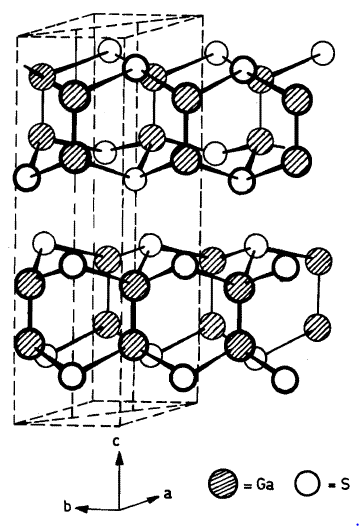
\includegraphics[width=0.5\linewidth]{Wlasciwosci/GaS_Schematic_Structure.png}
		\caption{Schematyczna reprezentacja struktury krystalicznej $\mathbf{GaS}$ [1]}
	\end{center}
\end{figure}
W kryształach $\mathbf{GaS}$ dominują słabe siły van der Waalsa w oddziaływaniach międzywarstwowych. Silne kowalencyjne siły dominują w oddziaływaniach wewnątrzwarstwowych.
$\mathbf{GaS}$ to półprzewodnik szerokopasmowy, który jest obiecującym materiałem. Skośna przerwa energetyczna wynosi $2.5eV$, a prosta wynosi $2.95eV$. Materiał umożliwia
wytwarzanie niebieskich urządzeń emitujących światło [1].

\newpage

\subsection{Siarczek galu(III)}
$\mathbf{Ga_{2}S_{3}}$ jest członkiem III-VI grupy związków chemicznych (III : In Ga VI : S, Se, Te), które mogą posiadać szeroką przerwę energetyczną. 
Nieścisłość pomiędzy atomami III i VI grupy zwykle powoduje, że związek III-VI ma różne stechiometrii, zróżnicowane fazy krystaliczne i różne formy sieci krystalicznej. Jest to półprzewodnik z prostą przerwą energetyczną 2-2.4 eV, i skośną przerwą energetyczną 2.5 - 3.4 eV. Takie rozbieżne wartości wynikają z
niepewności co do jakości kryształu i braku wiedzy struktury Ga2S3.

Struktura krawędzi pasma i pasmo wzbronione są kluczowymi parametrami dla funkcjonalnego półprzewodnika chalkogenkowego
jego zastosowania w optoelektronice, nanoelektronice i urządzeniach fotonicznych.

Materiał $\mathbf{Ga_{2}S_{3}}$ może występować w kilku fazach atomy w których tworzą układy: jednoskośny, heksagonalny, regularny. Może posiadać wadliwą strukturę blendy cynkowej w której $\frac{1}{3}$ miejsc kationowych są puste.
[001-Ga2S3-srep06143]

Faza jednoskośna: a = 1.114, b = 0.641, c = 0.703 nm, $\beta$ = 121.22$^\circ$.[004-Ga2S3-281 - Optik Ga2S3 8]

Znane trzy odmiany $\mathbf{Ga_{2}S_{3}}$:

1) Niskotemperaturowa. Kryształki białego koloru. Układ kubiczny grupa przestrzenna $\mathbf{F\;\overline{4}3m}$.

2) (faza $\beta$) Po podgrzaniu do 550-600$^\circ C$ przekształca się w żółtawą modyfikację, która
tworzy sześciokątną nieuporządkowaną strukturę (typu ZnS(Blenda cynkowa) lub wurcytu). Grupa przestrzenna $P63mc$

3) W temperaturze 600$^\circ C$ tworzą się zasadniczo przezroczyste i jasnożółte kryształki. Jednoskośna struktura. Dla tej struktury około 3.0 eV przerwa energetyczna.

Dla publikacji [001-Ga2S3-srep06143] znaleziono dla fazy jednoskośnej
a = 1.111 b = 0.958 c = 0.640 $\gamma$ = 141$^\circ$ Jednak pozycja znaczących pików na widmie XRD jest taka sama dla każdej fazy
różnica polega jedynie na zmianie względnej intensywności pików dla każdej fazy.
\textbf{Czy z tego wynika że i dla fazy jednoskośnej też są luki?}

Struktura wszystkich faz jest podobna i to jest struktura blendy cynkowej z luką galową na co trzeciej pozycji. Siarka zajmuje
pozycje prawie idealnie sześciokątnego opakowania i różne
uporządkowanie w podsieci kationowej powoduje polimorfizm.	 
[005-Ga2S3-1-s2.0-S0025540816307498-main]

$\mathbf{Ga_{2}S_{3}}$ tworzy jasnożółte kryształki układu jednoskośnego, grupa przestrzenna
$\mathbf{F\;\overline{4}3m}$.
\begin{figure}[H]
	\begin{center}
		\begin{minipage}[h]{0.3\linewidth}
			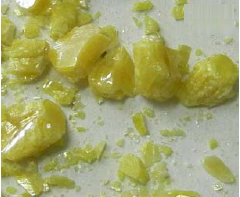
\includegraphics[width=1\linewidth]{Wlasciwosci/Ga2S3_View_Bridgman_Method.png}
		\end{minipage}
		\begin{minipage}[h]{0.3\linewidth}
			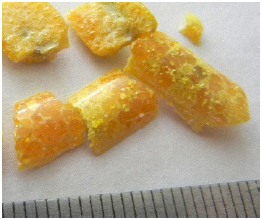
\includegraphics[width=1\linewidth]{Wlasciwosci/Ga2S3_View_Flux_Method.png}
		\end{minipage}
		\caption{Kryształki siarczku galu(III). Po lewej stronie $\mathbf{Ga_{2}S_{3}}$ wytworzony metodą Bridgmana. Po prawej $\mathbf{Ga_{2}S_{3}}$ wytworzony metodą flux-melt.[3]}
	\end{center}
\end{figure}
 Ze względu na budowę warstwową jest rozważany jako perspektywiczny materiał do zastosowań w nanoelektronice i fotonice oraz do generacji sygnałów THz.
 Kryształy $\mathbf{Ga_{2}S_{3}}$ mają również wysoką foto-wrażliwość i silną reakcję luminescencji. 
   Dodatkową jego zaletą jest silna anizotropia optyczna i jest rozważany jako materiał nieliniowy do generacji drugiej harmonicznej (SHG) w zakresie średniej podczerwieni.
\begin{figure}[H]
	\begin{center}
		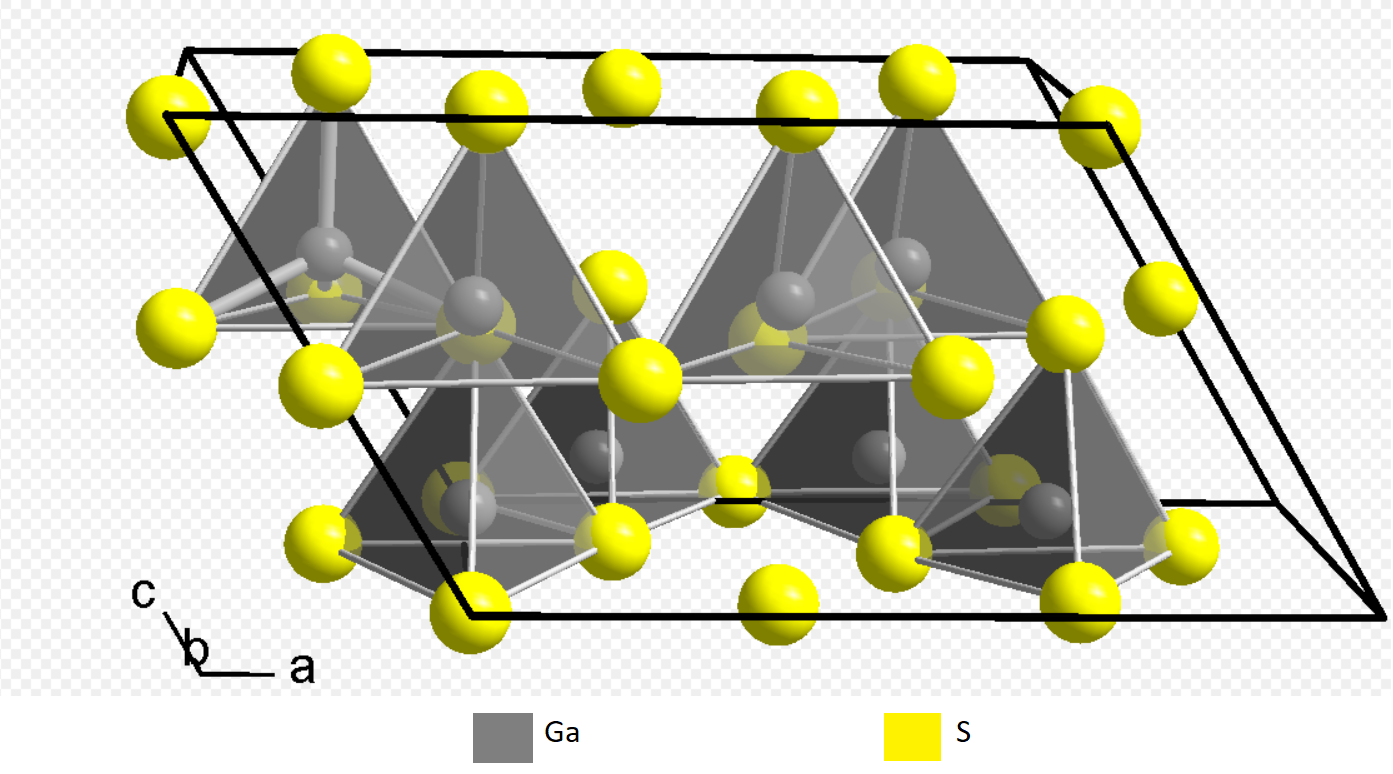
\includegraphics[width=0.6\linewidth]{Wlasciwosci/Ga2S3_Schematic_Structure2.png}
		\caption{Struktura krystaliczna $\mathbf{Ga_{2}S_{3}}$.[2]}
	\end{center}
\end{figure}




	\newpage

\section{Rozpraszanie Ramanowskie}
\subsection{Czym jest spektroskopia ramanowska}
Spektroskopia Ramana jest istotną metodą badania widm rotacyjnych i oscylacyjnych cząsteczek. Światło rozpraszane ma inne częstości niż światło padające. Obserwujemy przesunięcie linii zarówno w stronę większych jak i mniejszych częstości, a tym samym większych i mniejszych energii. Kilka cech tej spektroskopii jest niezwykle ważnych. Jedną z nich jest możliwość użycia światła widzialnego do badania widma Ramana. Można lepiej operować takim światłem w warunkach doświadczenia niż światłem podczerwonym lub mikrofalami. Niektóre dwuatomowe cząsteczki jak $\mathbf{H_{2}}$ czy $\mathbf{O_{2}}$ nie posiadają momentu dipolowego i dlatego nie są aktywne w podczerwieni, a ich widma mogą być badane właśnie w widmie Ramana. Zatem np. pod tym względem spektroskopia ramanowska jest dopełnieniem spektroskopii w podczerwieni i odwrotnie. Poza tym spektroskopia ramanowska umożliwia badanie ruchu cząsteczek, które zmieniając swoje położenie, wykonują np. ruchy obrotowe, co z kolei powoduje zmianę ich ukierunkowania względem padającego promieniowania. Objawia się to zmianą polaryzacji w stosunku do światła padającego. Ponadto rozpraszanie Ramana, podobnie jak spektroskopia w podczerwieni, dostarcza informacji o budowie cząsteczki, wiązaniach międzyatomowych, które ją tworzą, a także o ich polaryzowalności. Pozwala to przewidzieć reaktywność chemiczną i przebieg reakcji chemicznych.

Rozproszone fotony co mają określone przesunięcie energetyczne są parametrami do stwierdzenia rodzaju gazu. Aktywne przejścia Ramana, inne niz przejscia w podczerwieni. Wszystkie dwuatomowe gazy homonuklearne są niewidoczne w podczerwieni ($\mathbf{O_{2}}$, $\mathbf{N_{2}}$, $\mathbf{H_{2}}$, $\mathbf{Cl_{2}}$), a w widmie Ramana są widoczne. Dodatkową zaletą spektroskopii ramanowskiej jest to że można identyfikować mieszaninę gazów. Na podstawie tego jest zastosowanie: w wykrywaniu paliwa gazowego dla elektrowni naturalnych lub biogazowych, w których $\mathbf{CH_{4}}$, $\mathbf{CO_{2}}$, $\mathbf{O_{2}}$, $\mathbf{N_{2}}$ i $\mathbf{H_{2}}$ są istotne dla monitorowania, w procesach przemysłowych gdzie ma miejsce $\mathbf{H_{2}O}$, dla tego, że czujniki Ramana są słabo uszkadzane wodą. Pomiar odbywa się na bieżąco. Dalsze zalety czujników gazowych Ramana są w stanie tolerować wysokie stężenia gazu i mieć wysoki zakres dynamiczny, ponieważ nie cierpią z powodu efektów nasycenia. Objętość pomiaru może być bardzo mała w spektroskopii ramanowskiej. Pomiar w mikroreaktorach dla chemii kombinatorycznej. Główną wadą spektroskopii ramanowskiej jest to, że proces rozpraszania jest dość słaby, co oznacza, że jest trudny w uzyskaniu akceptowalnej czułości. Większość spektrometrów ramanowskich są zbudowane do wykrywania ciał stałych lub płynów, gdzie wyższa gęstość materiału znacząco zwiększa sygnał. 

\subsection{Wgląd matematyczny}
Jeżeli światło o natężeniu 
\begin{equation}
	E = E_{m}\cos (2\pi f_{p}t)
\end{equation}
\begin{itemize}
	\item[-]{$E$ - natężenie padającego światła};
	\item[-]{$E_{m}$ - wartość maksymalna natężenia};
	\item[-]{$f_{p}$ - częstotliwość promieniowania padającego}.
\end{itemize}
pada na cząsteczkę, to wystąpi oddziaływanie pomiędzy wektorem $\overrightarrow{E}$, a elektronowymi powłokami atomów tworzących cząsteczkę.
Elektrony w cząsteczkach wykazują polaryzowalność $\alpha$, czyli zdolność przemieszczania
się pod wpływem pola elektrycznego. W wyniku takiego przemieszczenia jest indukowany w cząsteczce moment dipolowy.
\begin{equation}
	p_{i} = \alpha E = E_{m}\cos (2\pi f_{p}t)
\end{equation}
Ponieważ ten moment dipolowy oscyluje z częstotliwością $f_{p}$ następuje emisja promieniowania o tej samej częstotliwości. Ta częstotliwość nosi nazwę 
\textit{rozpraszania Rayleigha}.

Niech cząsteczka wykonuje drgania z częstotliwością $f_{osc}$, to wychylenie z położenia 
równowagi można opisać wzorem:
\begin{equation}
	r - r_{0} = r_{m}\cos (2\pi f_{osc}t)
\end{equation}
\begin{itemize}
	\item[-]{$r_{0}$ - położenie równowagi};
	\item[-]{$r_{m}$ - maksymalne wychylenie};
	\item[-]{$f_{osc}$ - częstotliwość drgań cząsteczki}.
\end{itemize}
Polaryzowalność cząsteczki zmienia się wraz z odległością $r$. Ta wielkość może być
przedstawiona w postaci szeregu potęgowego:
\begin{equation}
	\alpha(r) = \alpha(r_{0}) + \frac{d\alpha}{dr}(r - r_{0}) + 
	\frac{d^{2}\alpha}{dr^{2}}(r - r_{0})^{2} + ... +
	\frac{d^{n}\alpha}{dr^{n}}(r - r_{0})^{n}
\end{equation}
W dalszych przekształceniach nie będziemy uwzględniać wyrazów rzędów wyższych od jednego. 

Uwzględniając wzory (1),(2),(3) możemy przedstawić moment dipolowy cząsteczki w następujący
sposób:
\begin{equation}
	p(t) = \alpha E = 
	\left\{ 
		\alpha(r_{0}) + \frac{d\alpha}{dr}r_{m}\cos (2\pi f_{osc}t) 
	\right\}
	E_{m}\cos (2\pi f_{p}t)
\end{equation}
Możemy przekształcić powyższe równanie po zastosowaniu wzoru na iloczyn cosinusów:
\begin{equation}
	p(t) = \alpha(r_{0})E_{m}\cos (2\pi f_{p}t) + \frac{d\alpha}{dr}E_{m}r_{m}
	\left\{
		\cos (2\pi (f_{p} + f_{osc})t) + \cos (2\pi (f_{p} - f_{osc})t)
	 \right\}
\end{equation}
Ponieważ argumenty funkcji $\cos$ zawierają częstotliwość $f = f_{p} \pm f_{osc}$, w widmie światła
rozproszonego ta częstotliwość będzie obserwowana. Wielkość przesunięcia jest cechą charakterystyczną danej cząsteczki. Lnie widma, które przesunięte w stronę mniejszych energii, są tzw. pasma stokesowskie, a w stronę większych energii – antystokesowskie.
\begin{figure}[H]
	\begin{center}
		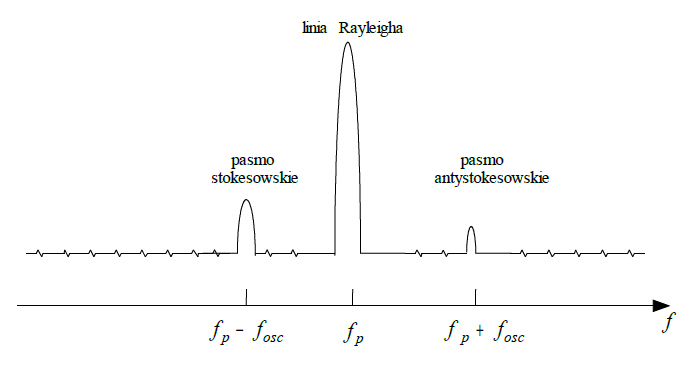
\includegraphics[width=1\linewidth]{Rozpraszanie-Ramanowskie/Schemat-widma-Ramanowskiego.png}
		\caption{Schemat widma ramanowskiego.[4]}
	\end{center}
\end{figure}

\subsection{Rodzaje pasm obserwowanych w widmie Ramana}
W widmie Ramana są obserwowane trzy rodzaje pasm:
\begin{itemize}
	\item[-]{Pasmo Rayleigha};
	\item[-]{Pasmo stokesowskie};
	\item[-]{Pasmo antystokesowskie}.
\end{itemize}

\textbf{Pasmo Rayleigha} - powstające na skutek oddziaływania fotonów padającego promieniowania o częstości $v_{0}$, nie pasujących do poziomów energetycznych cząsteczki. Po oddziaływaniu fotonu z cząsteczką, ostatnia wraca na ten sam poziom energetyczny.

\textbf{Pasmo stokesowskie} - gdy cząsteczka po oddziaływaniu z promieniowaniem przenosi się na wyższy poziom oscylacyjny i rozproszony foton ma energię mniejszą o różnicę energii poziomów oscylacyjnych $hv$.

\textbf{Pasma antystokesowskie} - jeśli przed oddziaływaniem z promieniowaniem molekuła znajdowała się na wzbudzonym poziomie oscylacyjnym, to oddziaływanie przenosi ją na podstawowy poziom oscylacyjny. Energia rozproszonego fotonu jest większa o różnicę energii poziomów oscylacyjnych $hv$. Pasmo antystokesowskie pojawia się w widmie Ramana po przeciwnej stronie co pasmo stokesowskie w stosunku do pasma Rayleigha. Pasmo to ma zwykle niższą intensywność niż pasma stokesowskie.
\begin{figure}[H]
	\begin{center}
		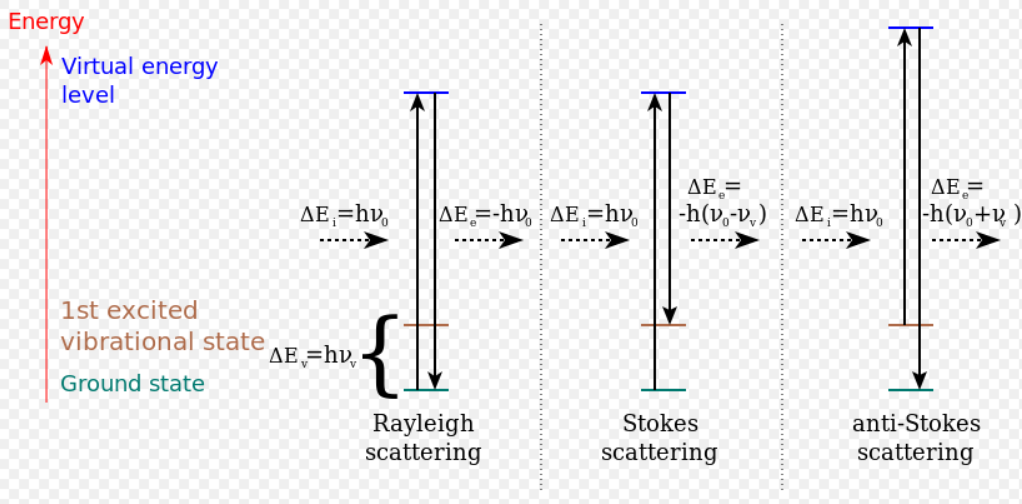
\includegraphics[width=1\linewidth]{Rozpraszanie-Ramanowskie/Raman-Energy.png}
		\caption{Diagram energii przejść w poszczególnych rodzajach rozpraszania.}
	\end{center}
\end{figure}
Widmo antystokesowskie jest mnie intensywne niż widmo stokesowskie. To jest spowodowane tym,
że prawdopodobieństwo oddziaływania fotonu ze wzbudzonym atomem jest dużo mniejsze niż
oddziaływanie z atomem w stanie podstawowym.

\subsection{Czynniki warunkujące zaistnienie zjawiska}
\subsubsection{Idealny dipol}
Przykładem takiego dipola może być układ składający się z spoczynkowego ładunku dodatniego $+Q$ i ładunku ujemnego $-Q$, harmonicznie oscylującego wzdłuż kierunku $\overrightarrow{P}$ z częstotliwością $\omega$.
\begin{equation}
	p = p_{0}\cos(\omega t)
\end{equation}
Problem promieniowania dipola ma istotne znaczenie w teorii układów promieniujących, ponieważ każdy rzeczywisty układ promieniujący (na przykład antena) może być obliczony na podstawie promieniowania dipola. Ponadto wiele pytań dotyczących interakcji promieniowania z materią można wyjaśnić na podstawie klasycznej teorii, biorąc pod uwagę atomy jako układy ładunków, w których elektrony wykonują oscylacje harmoniczne w pobliżu ich pozycji równowagi.

Jeśli fala rozchodzi się w homogenicznym ośrodku izotropowym, to czas przejścia fali do punktów odległych od dipola o odległość $r$ jest taki sam. Dlatego we wszystkich punktach kuli, której środek pokrywa się z dipolem, faza oscylacji jest taka sama, to znaczy w strefie falowej przód fali będzie sferyczny, a w konsekwencji fala emitowana przez dipol jest sferyczną falą.

W każdym punkcie wektory $\overrightarrow{E}$ i $\overrightarrow{H}$ oscylują zgodnie z prawem $\cos(\omega t - kr)$, amplitudy tych wektorów są proporcjonalne do
$\frac{\sin \theta}{r}$ (dla próżni). Czyli one zależą od odległości od $r$ odległości od środka dipola i kąta $\theta$ między kierunkiem momentu dipolowego i kierunkiem promieniowania.
\begin{figure}[H]
	\begin{center}
		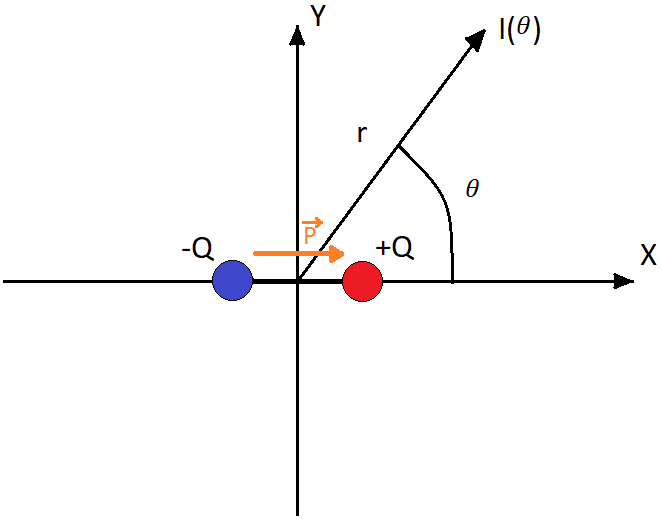
\includegraphics[width=0.6\linewidth]{Rozpraszanie-Ramanowskie/Point-Dipol.png}
		\caption{Drgający dipol, który twarzą dwa ładunki $-Q$ i $+Q$. $I(\theta)$ to jest natężenie promieniowania na odległości $r$ pod kątem $\theta$.}
	\end{center}
\end{figure}
Wynika stąd, że natężenie promieniowania dipolowego wynosi:
\begin{equation}
	I \sim \frac{\sin^{2}\theta}{r^{2}}
\end{equation}
Dla $\theta = \frac{\pi}{2}$ intensywność promieniowania jest maksymalna, a dla 
$\theta = 0$ i $\theta = \pi$ jest minimalna i wynosi $0$. Czyli dipol nie promieniuje wzdłuż kierunku momentu dipolowego.
\subsubsection{Realny dipol}
Warunkiem zaistnienia zjawiska Ramana są zmiany polaryzowalności cząsteczki w trakcie danego drgania. Polaryzowalność jest wielkością, którą można wyrazić za pomocą tensora, który jest układem 9 współczynników:
\begin{equation}
	\alpha = 
	\begin{vmatrix}
	\alpha_{xx} & \alpha_{xy} & \alpha_{xz} \\
	\alpha_{yx} & \alpha_{yy} & \alpha_{yz} \\
	\alpha_{zx} & \alpha_{zy} & \alpha_{zz}
	\end{vmatrix}
\end{equation}
Gdy mówimy np. o indukowanym momencie dipolowym, to pierwszy wskaźnik dwuelementowego indeksu oznacza kierunek momentu dipolowego, a drugi kierunek przyłożonego pola elektrycznego (wektora natężenia pola).

\newpage
\subsection{Przykładowe widma ramanowskie}
Widmo ramanowskie dla materiałów $GaS$ i $Ga_{2}S_{3}$:
\begin{figure}[H]
	\begin{center}
		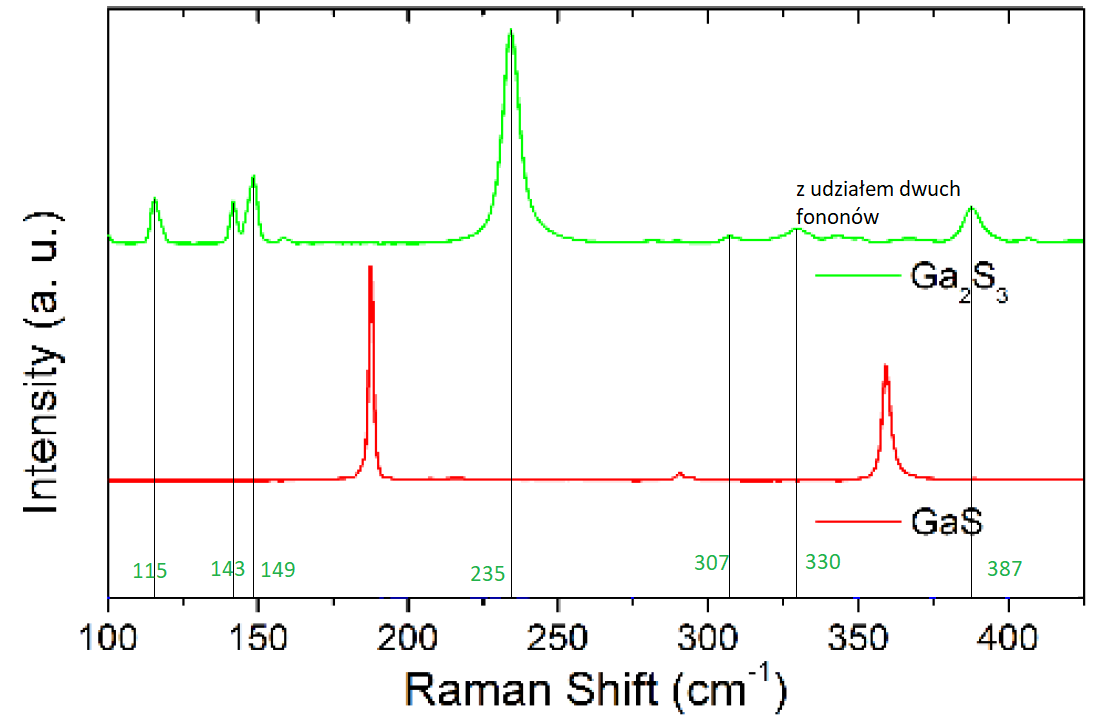
\includegraphics[width=0.8\linewidth]{Rozpraszanie-Ramanowskie/Raman-Shift.png}
		\caption{Widma rozpraszania ramanowskiego dla materiałów $GaS$ i $Ga_{2}S_{3}$[3]}
	\end{center}
\end{figure}
Na powyższym rysunku pokazane tylko pasma stokesowskie, ponieważ tylko tą częścią będę się zajmował w swojej pracy.

Energia fotonu wynosi:
\begin{equation}
	E = h \nu = h \frac{c}{\lambda} = hc \frac{1}{\lambda} 
\end{equation}
\begin{itemize}
	\item[-]{$h$ - stała Plancka};
	\item[-]{$c$ - prędkość światła};
	\item[-]{$\lambda$ - długość fali}.
\end{itemize}
Czyli odwrotność długości jest proporcjonalna do energii:
\begin{equation}
	\lambda^{-1} \sim E
\end{equation}

Zeru na powyższym widmie odpowiada energia światła pobudzającego (lasera) z przesunięciem wynoszącym zero. Czyli przesunięcie w widmie stokesowskim można zapisać w następując sposób:
\begin{equation}
	\frac{1}{\lambda} = \left| \frac{1}{\lambda_{Laser}} - \frac{1}{\lambda_{stok}} \right|
\end{equation}
\begin{itemize}
	\item[-]{$\lambda_{Laser}$ - długość fali promieniowania laserowego};
	\item[-]{$\lambda_{stok}$ - długość fali promieniowania stokesowskiego}
\end{itemize}














	\newpage

\section{Rozpraszanie Ramanowskie w ciękich warstwach}
\subsection{Fonony w materiale}
\textbf{Fonon} -  kwazicząstka, kwant energii drgań sieci krystalicznej. Są dwa rodzaje fononów:
\begin{itemize}
	\item{Fonony akustyczne. Powstają w wyniku drgań jednego rodzaju atomów.}
	\item{Fonony optyczne. Powstają w wyniku drgań różnego rodzaju atomów.}
\end{itemize}
Podział fononów jest uzależniony od kształtu relacji dyspersji w pobliżu k=0. \\
Fonony akustyczne wykazują zależność:
\begin{equation}
	\lim_{k \to 0} \omega(k) = 0
\end{equation}
natomiast fonony optyczne:
\begin{equation}
\lim_{k \to 0} \omega(k) = const
\end{equation}
\begin{figure}[H]
	\begin{center}
		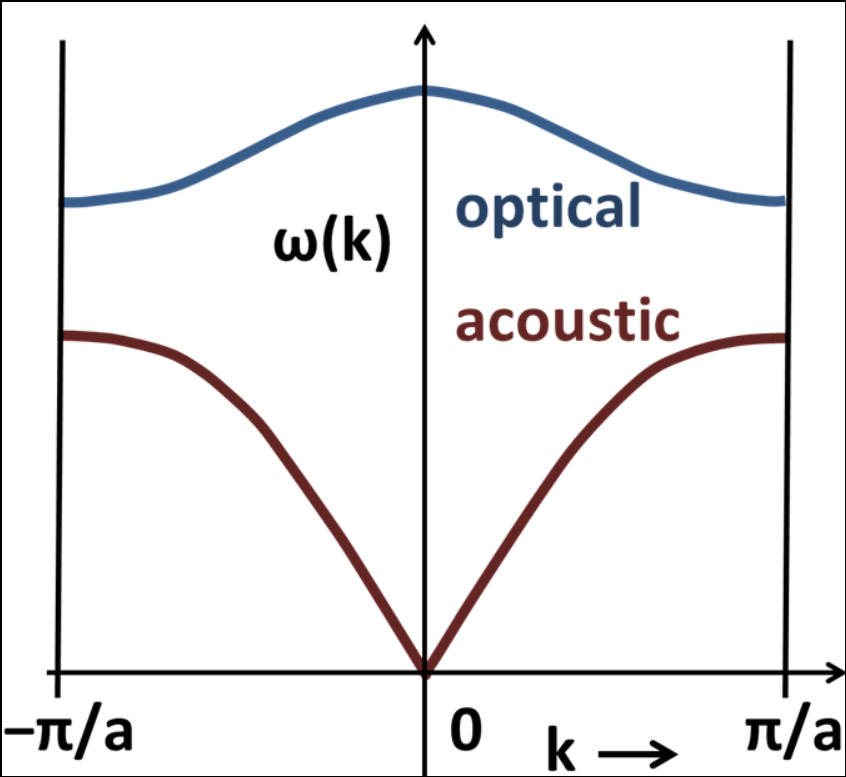
\includegraphics[width=0.8\linewidth]{Rozpraszanie-Ramanowskie-Ciekie/Phonons.png}
		\caption{Krzywe dyspersyjne dla liniowego łańcucha dwuatomowego.[5]}
	\end{center}
\end{figure}
Dla kryształu zawierającego N(>2) różnych atomów w komórce prymitywnej relacja dyspersji zawiera trzy gałęzie akustyczne oraz $\alpha$N-3 gałęzie optyczne, gdzie $\alpha$ to jest wymiar. Więc dla liniowego łańcucha dwuatomowego N=2 mamy jedną gałąź optyczną i jedną akustyczną. A dla trójwymiarowej komórki prostej składającej się z dwóch różnych cząsteczek będą 3 krzywe optyczne i 3 akustyczne.

Przy rozpraszaniu fotonów na fononach powinny być spełnione dwa prawa zachowania: 

Prawo zachowania energii:
\begin{equation}
	\hbar \mathbf{\omega_{i}} = \hbar \mathbf{\omega_{s}} \pm \hbar \mathbf{\Omega_{fonon}}
\end{equation}
\begin{itemize}
	\item $\omega_{i}$ - częstotliwość fotonu padającego;
	\item $\omega_{s}$ - częstotliwość fotonu rozproszonego;
	\item $\Omega_{fonon}$ - częstotliwość fononu;
	\item $\hbar$ - stała Plancka.
\end{itemize}

Prawo zachowania pędu:
\begin{equation}
	\hbar \mathbf{k_{i}} = \hbar \mathbf{k_{s}} \pm \hbar \mathbf{K_{fonon}}
\end{equation}
\begin{itemize}	
	\item $k_{i}$ - wektor falowy fotonu padającego;
	\item $k_{s}$ - wektor falowy fotonu rozproszonego;
	\item $K_{fonon}$ - wektor falowy fononu;
	\item $\hbar$ - stała Plancka.
\end{itemize}

Pęd fononu jest znacznie większy od pędu fotonu, a energia fotonu jest 
znacznie większa od energii fononu. To znaczy że uczęstniczą w oddziaływaniu tylko te 
fonony co mają mały pęd.

\begin{figure}[H]
	\begin{center}
		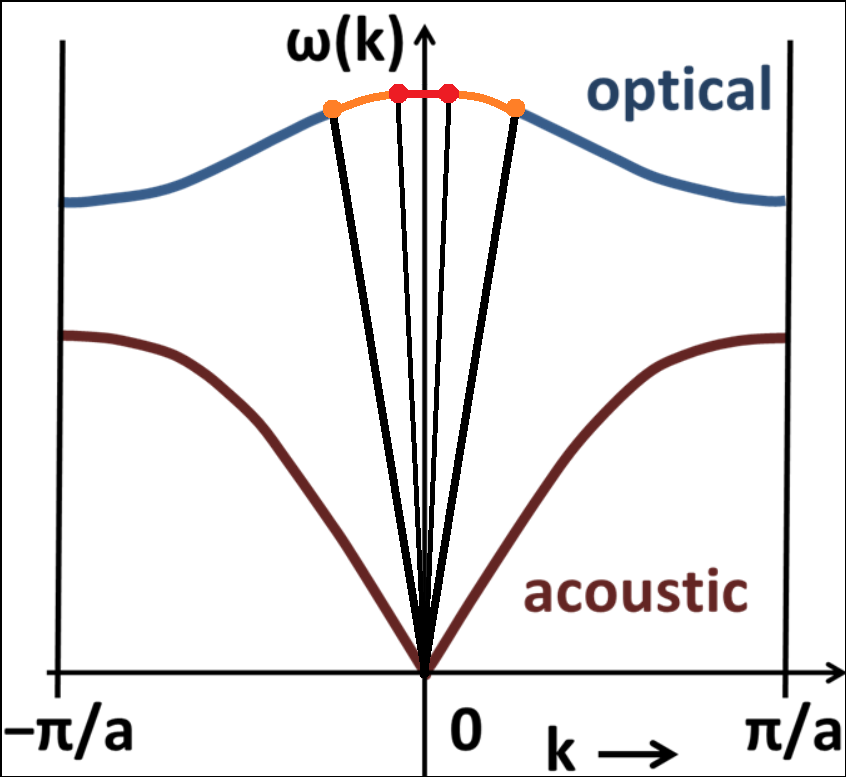
\includegraphics[width=0.8\linewidth]{Rozpraszanie-Ramanowskie-Ciekie/PhononsCenter.png}
		\caption{Krzywe dyspersyjne z zaznaczonym obszarem pokazującym które fonony uczęstniczą w rozpraszaniu ramanowskim.}
	\end{center}
\end{figure}

Z powyższego rysunku widzimy, że w oddziaływaniach przyjmują udział tylko optyczne fonony co znajdują się w środku strefy Brillouina. Akustyczne fonony nie biorą udziału dlatego, że dla $k \rightarrow 0$ energia też dąży do zera.

\vspace{1cm}
W niniejszej pracy były badane tylko widma stokesowskie dla tego, że one są bardziej intensywne niż widma antystokesowskie. Miarą intensywności widma są piki, które uzyskujemy. Im większe piki, tym mniejszy błąd przy analizie wyników pomiaru.
Prawdopodobieństwo obsadzenia stanu energetycznego fononem jest proporcjonalne do:
\begin{equation}
	\sim \exp^{-\frac{E}{kT}} 
\end{equation}
\begin{itemize}
	\item{$E$ - energia stanu energicznego};
	\item{$k$ - stała Boltzmanna};
	\item{$T$ - temperatura w Kelwinach}.
\end{itemize}
to znaczy że stosunek intensywności promieniowania rozproszonego w widmie antystokesowskim
do intensywności promieniowania pobudzającego jest:
\begin{equation}
	\frac{I_{ants}}{I} \sim \exp^{-\frac{E}{kT}}
\end{equation}
\begin{itemize}
	\item{$I_{ants}$ - intensywność promieniowania w widmie antystokesowskim};
	\item{$I$ - intensywność promieniowania pobudzającego}
\end{itemize}
	Typowa energia wzbudzenia fononu $E = 0.065eV$, więc:
\begin{equation}
	\sim \exp^{-\frac{E}{kT}} = \exp^{-\frac{0.065}{0.025}} \approx 0.07
\end{equation}
Czyli intensywność widma antystokesowskiego wynosi $7\%$ widma stokesowskiego. 
\subsection{Co można odczytać z widma Ramanowskiego}
Ważną rolę w widmie Ramanowskim odgrywa szerokość połówkowa pików.
Na podstawie informacji o szerokości połówkowej $\Gamma$ można mówić o czasie życia fononów w próbce:
\begin{equation}
	\Gamma \sim \frac{1}{\tau}
\end{equation}

gdzie $\tau$ - czas życia fononu.

\begin{figure}[H]
	\begin{center}
		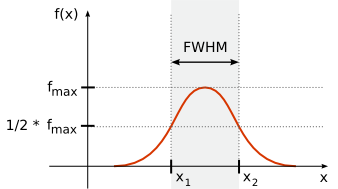
\includegraphics[width=0.8\linewidth]{Full_width_at_half_maximum.png}
		\caption{Szerokość połówkowa piku \textit{FWHM} - z angielskiego \textit{Full Width at Half Maximum}.}
	\end{center}
\end{figure}

Szerokość połówkowa zależy od:
\begin{itemize}
	\item[1]{Rozmiar próbki. Czy materiał jest cienkowarstwowym, czy bulk.}
	\item[2]{Defekty. Fonony rozpraszają się na defektach, co zmniejsza czas ich życia.}
	\item[3]{Rozpraszanie fononów wskutek efektów anharmonicznych}
\end{itemize}
Na podstawie szerokości piku można uzyskać informację o przewodnictwie cieplnym próbki. 
W zależności od ilości i kształtu pików można zbadać jaki to jest materiał, czy badany materiał jest czystym materiałem bez domieszek.
Na podstawie widma Ramanowskiego można oszacować temperaturę ciała. Czyli jest możliwy pomiar temperatury bez ingeracji do badanego materiału.

\subsection{Piki ramanowskie w cienkich warstwach}
W materiałach cienkowarstwowych jeden z wymiarów jest rzędu kilku nanometrów. To powoduje że zaczynają odgrywać ważną rolę efekty kwantowe. Z zasady nieoznaczoności Heisenberga:
\begin{equation}
	\Delta p_{fon} \Delta d \geq \frac{\hbar}{2}
\end{equation}
\begin{itemize}
	\item{$\Delta p_{fon}$ - niepewność pomiaru pędu fononu};
	\item{$\Delta d$ - niepewność pomiaru położenia fononu}
\end{itemize}
\textbf{ZAPYTAĆ!jak przejść z tej regóły do kształtu piku}
Pik jest rozmazany w kierunku wyższych energii.
\\
RYSUNEK PIKU ROZMAZANEGO
\\

Napisać o rozpraszaniu dwufononowym

\subsection{Dane dla pików ramanowskich GaP Ga2S3}

\subsection{przyrząd pomiarowy, rysunek, opis}

	\newpage

\section{Przygotowanie próbek do badań}

\subsection{Przyrząd pomiarowy, rysunek, opis}
\begin{figure}[H]
	\begin{center}
		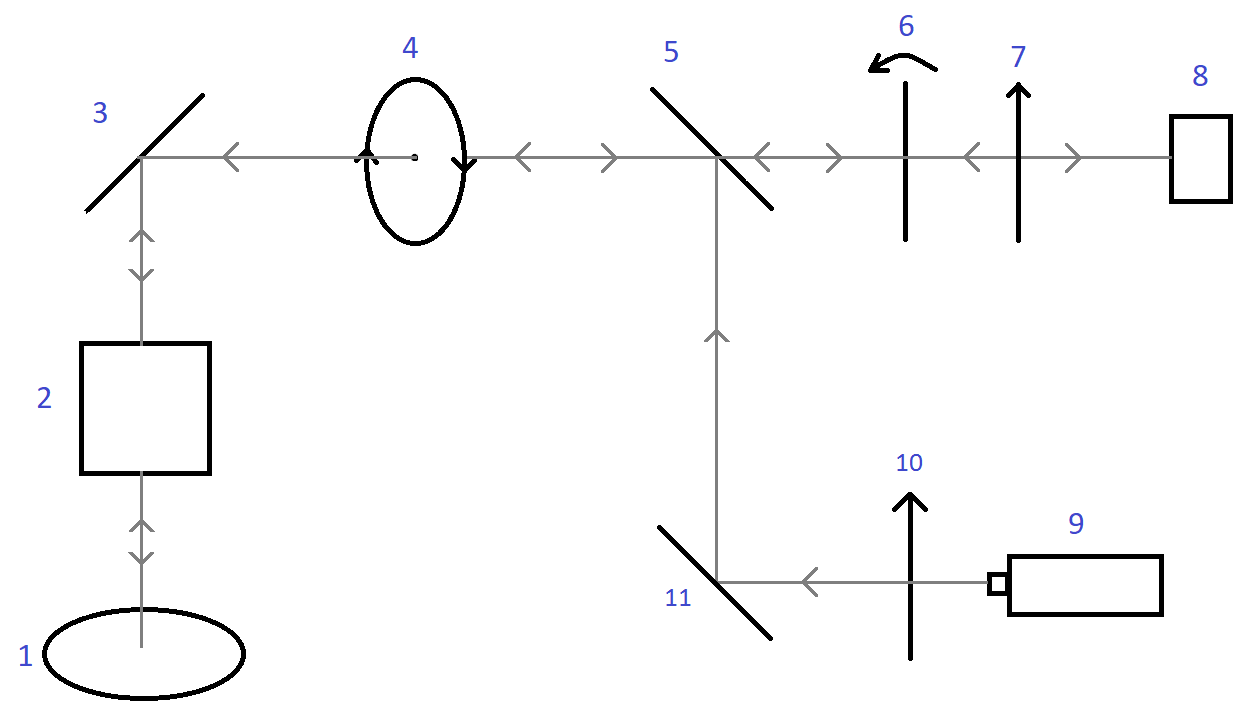
\includegraphics[width=1.0\linewidth]{Przygotowania/Uklad-pomiarowy.png}
		\caption{Schemat układu pomiarowego.}
	\end{center}
\end{figure}

\begin{itemize}
	\item 1 - Badana próbka, $\alpha$-$\mathbf{Ga_{2}S_{3}}$;
	\item 2 - Mikroskop;
	\item 3, 11 - Lustra;
	\item 4 - HWP\footnote{HWP z angielskiego ''Half-wave plate'' czyli  płytka półfalowa}, nazwa skrócona ''półfalówka'';
	\item 5 - Płytka pólprzepuszczająca;
	\item 6 - HWP 90$^{\circ}$, ustawiona tak że przekręca polaryzację o 90$^{\circ}$;
	\item 7, 10 - Polaryzatory;
	\item 8 - Detektor;
	\item 9 - Laser argonowy 514 nm;
\end{itemize}

Promieniowanie elektromagnetyczne o długości fali 514 nm, emitowane laserem argonowym (9), przechodzi przez pionowo ustawiony polaryzator (10). Chociaż fala elektromagnetyczna emitowana laserem już jest spolaryzowana, polaryzator (10) zapewnia dodatkową polaryzację. Dalej fala elektromagnetyczna odbija się od zwierciadła (11) i trafia na płytkę półprzepuszczającą (5). Zatem odbija się od tej płytki i przechodzi przez HWP (4), gdzie polaryzacja skręcona o określony kąt $\alpha$, po przejściu przez (4) polaryzacja fali elektromagnetycznej jest przekręcona o kąt 2$\alpha$. Dalej fala trafia na próbkę (1) przez (2). Rozproszona fala elektromagnetyczna na fononach trafia na zwierciadło (3), odbija się od tego zwierciadła i przechodzi prze ''półfalówkę'' (4). Teraz ''półfalówka'' względem światła rozproszonego ma skręcony kąt o $-\alpha$. Po przejściu przez (4) polaryzacja rozproszona fala elektromagnetycznej jest skręcona o -2$\alpha$. Dalej światło rozproszone trafia do ''półfalówki'' na stale przekręconej o 45$^\circ$ czyli fala, która przeszła przez (6) ma skręcony kąt polaryzacji o 90$^\circ$. Następnie po przejściu polaryzatora (7) fala elektromagnetyczna trafia na detektor z kamerą CCD. Polaryzator (7) jest po to aby zbierać światło rozproszone tylko o określonej polaryzacji.

Pomiar się odbywał w dwóch konfiguracjach:
\begin{itemize}
	\item VV - zbierane światło rozproszone w takim samym kierunku jak światło pobudzające\footnote{Światło emitowane laserem}. Bez HWP 90$^{\circ}$.
	\item VH - zbierane światło rozproszone w kierunku prostopadłym do światła pobudzającego. Z obecnością HWP 90$^{\circ}$.
\end{itemize} 

Charakterystyki pomiaru:
\begin{itemize}
	\item Czas pomiaru 30 sek;
	\item Środek detektora 1040 $cm^{-1}$;
	\item Moc lasera 10 \% z $\frac{3}{4}$ mocy maksymalnej;
	\item Polaryzacja lasera normalna;
	\item Długość fali 514 nm;
	\item Każdy pomiar skręcenie "półfalówki" co 5$^{\circ}$;
	\item Konfiguracja VV bez elementu (6) rys. 22. Konfiguracja VH z elementem (6).
	\item Oprogramowanie \textit{Wire} 4.2.
\end{itemize}

\textbf{\textcolor{red}{Zdjęcie i opis sprzętu pomiarowego, razem z oprogramowaniem}}.

Przy pomiarach powstawały niektóre trudności.

Płytka $\mathbf{GaP}$ ma wymiary 3mm x 2mm x 1mm. Kryształki które zostały utworzone na tej płytce były rzędu kilku mikrometrów. Poszukiwany kryształek do badań powinien przypominać sześciokąt, być osobnym kryształkiem i mieć płaską powierzchnię. Ta powierzchnia powinna być w miarę równoległa do podłoża.

Kryształki zostały utworzone na podłożu z $\mathbf{GaP}$. Piki na widmie ramanowskim pochodzące z galu nakładają się na niektóre piki pochodzące z $\mathbf{Ga_{2}S_{3}}$. To bardzo utrudnia analizę niektórych pików z $\mathbf{Ga_{2}S_{3}}$.

Kryształki zostały zdrapane papierem ściernym i przełożone na taśmę klejącą. Ale po kilku pomiarach ciepło które pochodzi od tego, że promieniowanie laserowe grzeje miejsce w które trafia. Taśma klejąca pod wpływem ciepła rozszerza się, co powoduje znaczącą rozkalibrację układu pomiarowego. 

Zostało podjęte ryzyko, że zdrapane kryształki należy przenieść na szklaną płytkę. Z tej płytki te kryształki można łatwo zdmuchnąć. To jest niebezpieczne dla tego, że cały pomiar może być robiony przez dwa dni po kilku godzin.

\subsection{Technologia wzrostu kryształków} 

$\mathbf{Ga_{2}S_{3}}$ posiada odmienną strukturę krystaliczną od $\mathbf{GaS}$ – żadna faza krystaliczna siarczku galu(III) nie wykazuje budowy warstwowej. W związku z tym otrzymywanie cienkich warstw $\mathbf{Ga_{2}S_{3}}$ nie jest możliwe w procesie eksfoliacji i wymaga zastosowania innych metod (np. CVD, MBE).

Warstwy $\mathbf{Ga_{2}S_{3}}$ były otrzymywane poprzez reakcję małych ilości par siarki z płytkami krystalicznego fosforku galu, które zostały wypolerowane z jednej strony.

W ampule kwarcowej umieszczono krystaliczną płytkę $\mathbf{GaP}$ \footnote{Płytka jest mała o wymiarach 5 x 3 x 1 mm.} oraz 1 mg krystalicznej siarki. Ampułę następnie zamknięto pod próżnią (<1 mbar) i wstawiono do pieca rurowego w taki sposób by płytka była w środku strefy grzejnej, a następnie rozpoczęto ogrzewanie ze wzrostem temperatury $1^{\circ}/min$ aż do osiągnięcia temperatury 600$C^{\circ}$
Reakcję prowadzono przez 4 dni, po których piec wyłączono i pozostawiono do naturalnego wystygnięcia.

Próbki były robione w ramach współpracy z wydziałem chemicznym w laboratorium wydziału chemicznego Politechniki Warszawskiej.

\begin{figure}[H]
	\begin{minipage}[h]{0.5\linewidth}
		\center{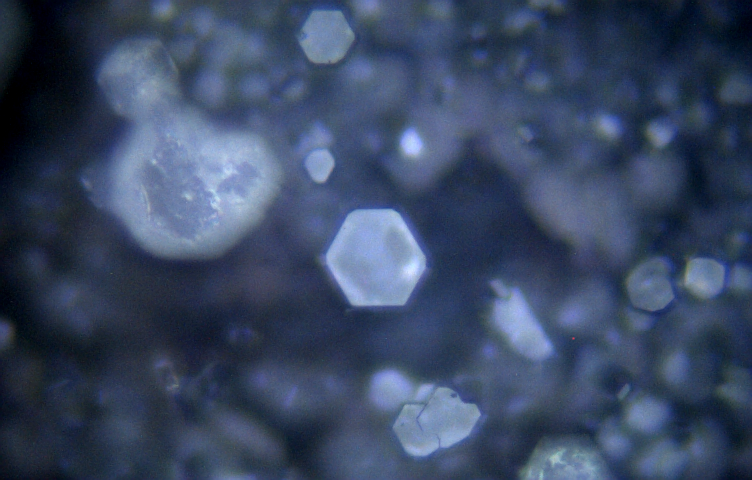
\includegraphics[width=0.8\linewidth]{Przygotowania/SLA39-50x-plytkiGa2S3.png}} \\ a) 
	\end{minipage}
	\hfill
	\begin{minipage}[h]{0.5\linewidth}
		\center{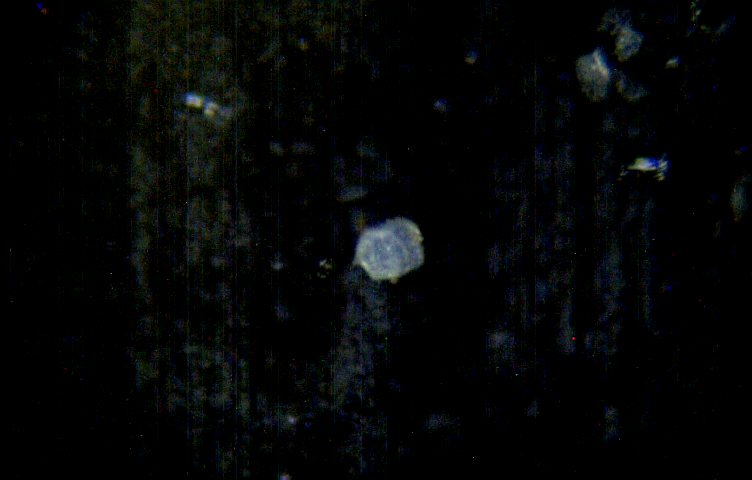
\includegraphics[width=0.8\linewidth]{Przygotowania/long50x.png}} \\b)
	\end{minipage}
	\caption{Kryształki badanego materiału $\mathbf{Ga_{2}S_{3}}$.}
\end{figure}

\begin{figure}[H]
	\begin{center}
		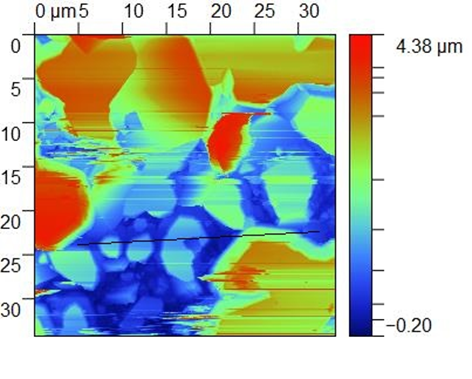
\includegraphics[width=0.65\linewidth]{Przygotowania/SEM.png}
		\caption{Skan typowej powierzchni uzyskanej w procesie syntezy.[36]}
	\end{center}
\end{figure}
























 
	\newpage

\section{Wyniki badań}

Pierwszy pomiar widma ramanowskiego został zrobiony dla kryształka, który był na podłożu $\mathbf{GaP}$. Wzrost kryształków się odbywał na tym podłożu. 

\begin{figure}[H]
	\begin{center}
		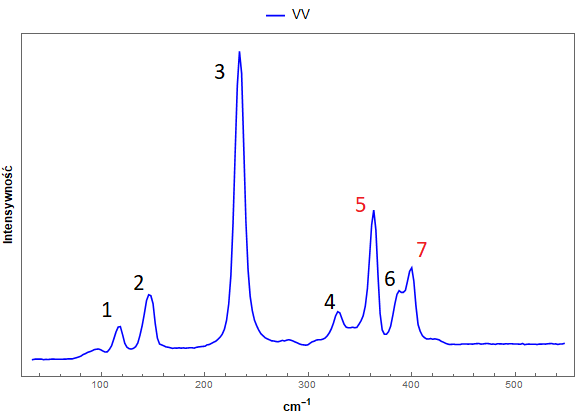
\includegraphics[width=0.8\linewidth]{Wyniki/Raman/plotGapWithGa2S3.png}
		\caption{Widmo ramanowskie dla $\mathbf{Ga_{2}S_{3}/GaP}$}
	\end{center}
\end{figure}

Piki 1,2,3,4,6 odpowiadają widmu ramanowskiemu dla $\mathbf{Ga_{2}S_{3}}$, a piki 5,7 odpowiadają widmu ramanowskiemu dla $\mathbf{GaP}$. Piki pochodzące z $\mathbf{GaP}$ znacznie utrudniają analizę piku 4 i 6. A poza tym można przypuszczać, że nie wszystkie piki, odpowiadające $\mathbf{Ga_{2}S_{3}}$ są widoczne z powodu obecności pików o numerach 5 i 7. 

Pomiary dla $\mathbf{Ga_{2}S_{3}/GaP}$ zostały zrobione tylko w konfiguracji VV, dlatego że później zostało postanowiono przenieść kryształki na inną powierzchnię aby pozbyć się niepożądanych pików na widmie ramanowskim. 

\newpage

Żeby to potwierdzić zostało uzyskane widmo ramanowskie dla $\mathbf{GaP}$, które pokazano na rysunku niżej:

\begin{figure}[H]
	\begin{center}
		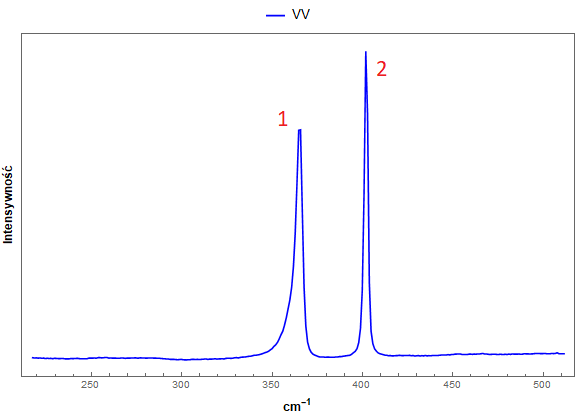
\includegraphics[width=0.8\linewidth]{Wyniki/Raman/plotGaP.png}
		\caption{Widmo ramanowskie dla $\mathbf{GaP}$. Piki 1 odpowiada przeunięciu około 360$cm^{-1}$, 2 -- 400$cm^{-1}$.}
	\end{center}
\end{figure}

\begin{figure}[H]
	\begin{minipage}[h]{0.5\linewidth}
		\center{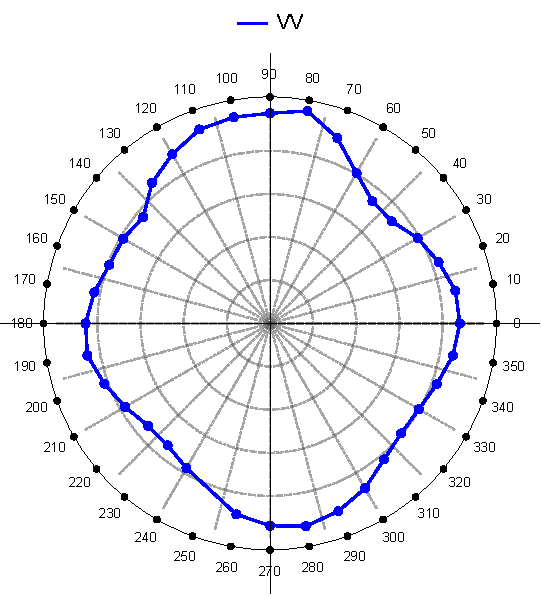
\includegraphics[width=0.8\linewidth]{Wyniki/WidmoPolaryzacyjne/plot5GaP.pdf}} \\ a) 
	\end{minipage}
	\hfill
	\begin{minipage}[h]{0.5\linewidth}
		\center{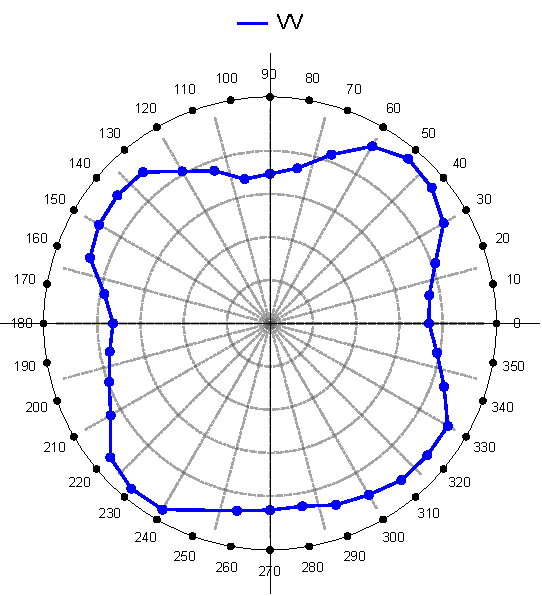
\includegraphics[width=0.8\linewidth]{Wyniki/WidmoPolaryzacyjne/plot7GaP.pdf}} \\b)
	\end{minipage}
	\caption{Widmo polaryzacyjne dla pików $\mathbf{GaP}$. a) Odpowiada piku 1, b) Odpowiada piku 2.}
\end{figure}

Po zdrapaniu kryształków na szkło zostało uzyskane następujące widmo ramanowskie:

\begin{figure}[H]
	\begin{center}
		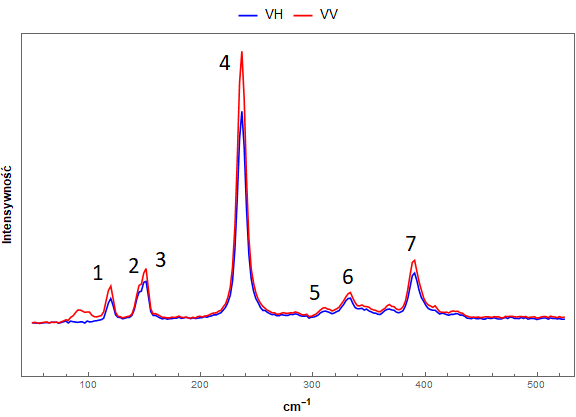
\includegraphics[width=0.8\linewidth]{Wyniki/Raman/plotVVandVH.png}
		\caption{Widmo ramanowskie dla $\mathbf{Ga_{2}S_{3}}$ bez wpływu $\mathbf{GaP}$ dla konfiguracji VV i VH.}
	\end{center}
\end{figure}

Na powyższym widmie ramanowskim zostały wyróżnione 7 pików. 1 $\rightarrow$ 117$cm^{-1}$, 2 $\rightarrow$ 143$cm^{-1}$, 3 $\rightarrow$ 149$cm^{-1}$, 4 $\rightarrow$ 235$cm^{-1}$, 5 $\rightarrow$ 309$cm^{-1}$, 6 $\rightarrow$ 330$cm^{-1}$, 7 $\rightarrow$ 390$cm^{-1}$. 

\begin{figure}[H]
	\begin{center}
		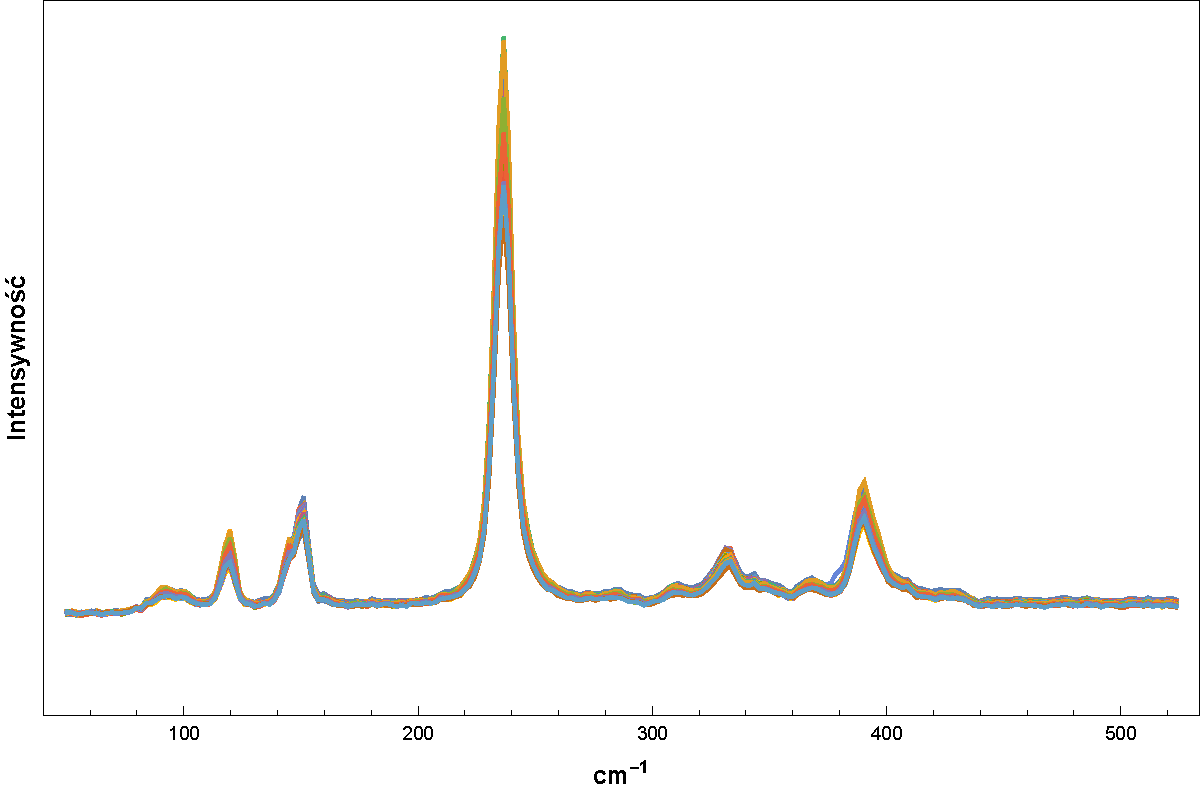
\includegraphics[width=0.8\linewidth]{Wyniki/Raman/plotAllVV.pdf}
		\caption{Widma ramanowskie dla 36 różnych kątów polaryzacji dla konfiguracji VV.}
	\end{center}
\end{figure}

\begin{figure}[H]
	\begin{center}
		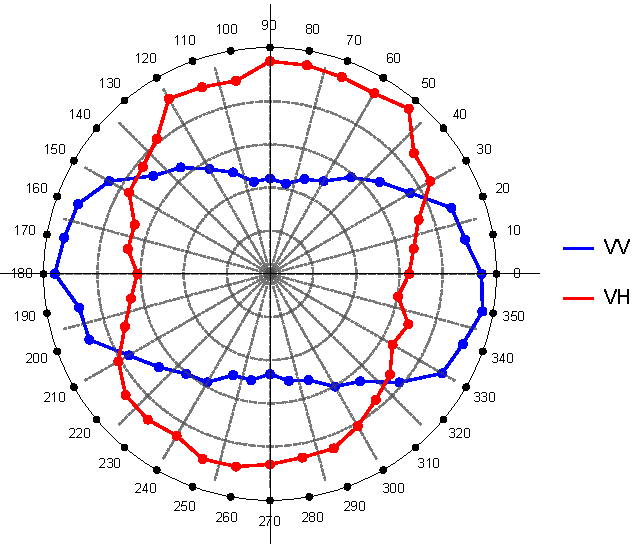
\includegraphics[width=0.75\linewidth]{Wyniki/WidmoPolaryzacyjne/plot117.pdf}
		\caption{Widmo polaryzacyjne dla pika 1 $\rightarrow$ 117$cm^{-1}$ }
	\end{center}
\end{figure}

\begin{figure}[H]
	\begin{center}
		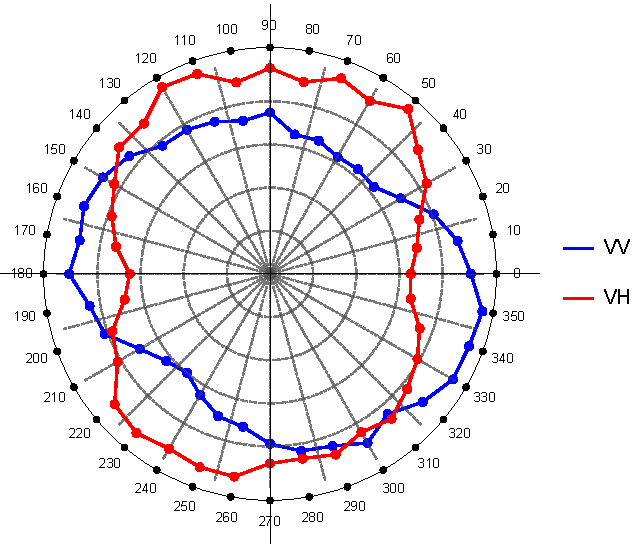
\includegraphics[width=0.75\linewidth]{Wyniki/WidmoPolaryzacyjne/plot143.pdf}
		\caption{Widmo polaryzacyjne dla pika 2 $\rightarrow$ 143$cm^{-1}$ }
	\end{center}
\end{figure}

\begin{figure}[H]
	\begin{center}
		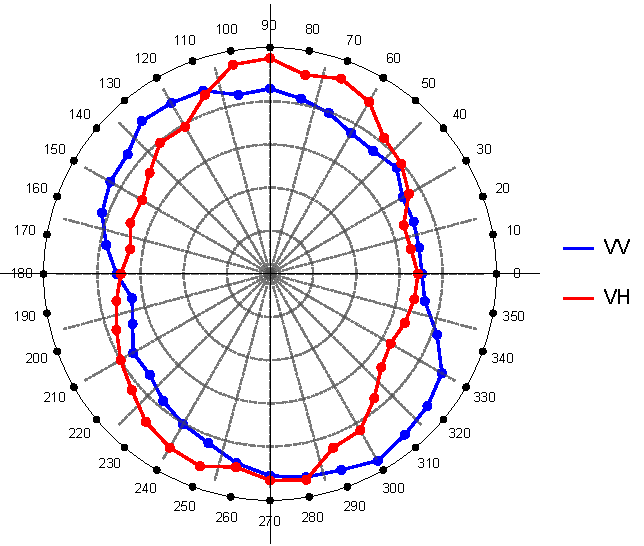
\includegraphics[width=0.75\linewidth]{Wyniki/WidmoPolaryzacyjne/plot149.pdf}
		\caption{Widmo polaryzacyjne dla pika 3 $\rightarrow$ 149$cm^{-1}$ }
	\end{center}
\end{figure}

\begin{figure}[H]
	\begin{center}
		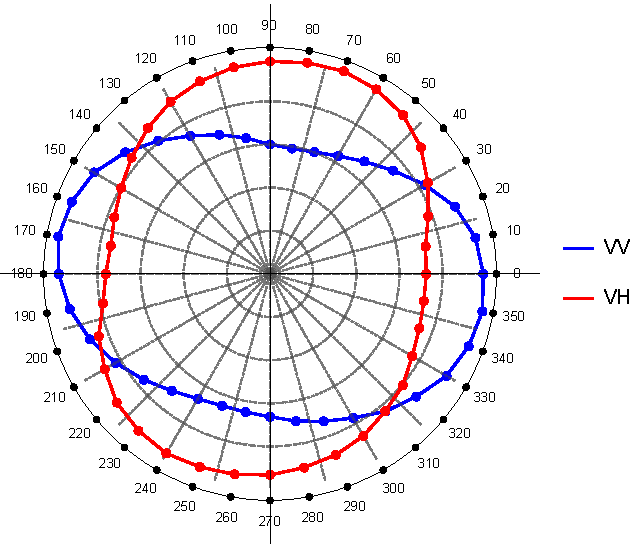
\includegraphics[width=0.75\linewidth]{Wyniki/WidmoPolaryzacyjne/plot235.pdf}
		\caption{Widmo polaryzacyjne dla pika 4 $\rightarrow$ 235$cm^{-1}$ }
	\end{center}
\end{figure}

\begin{figure}[H]
	\begin{center}
		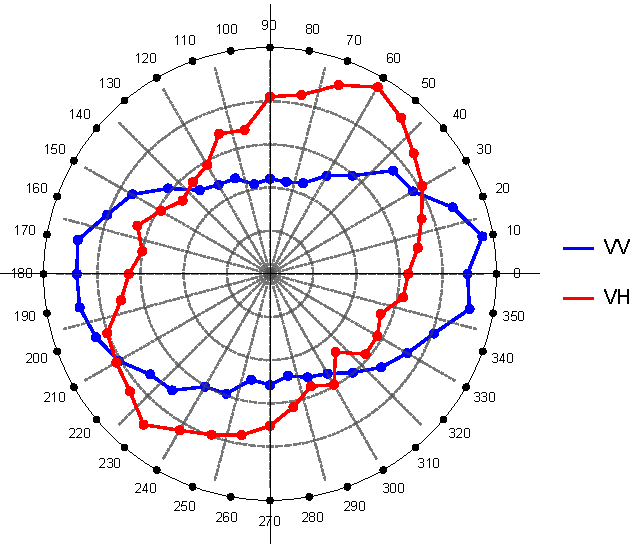
\includegraphics[width=0.75\linewidth]{Wyniki/WidmoPolaryzacyjne/plot309.pdf}
		\caption{Widmo polaryzacyjne dla pika 5 $\rightarrow$ 309$cm^{-1}$ }
	\end{center}
\end{figure}

\begin{figure}[H]
	\begin{center}
		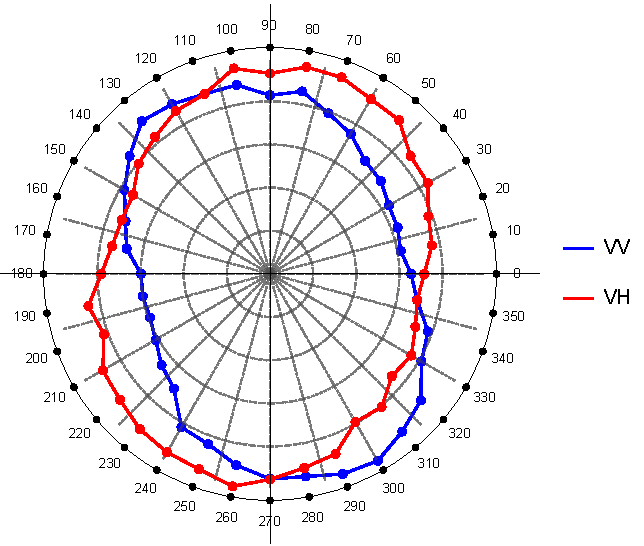
\includegraphics[width=0.75\linewidth]{Wyniki/WidmoPolaryzacyjne/plot330.pdf}
		\caption{Widmo polaryzacyjne dla pika 6 $\rightarrow$ 330$cm^{-1}$ }
	\end{center}
\end{figure}

\begin{figure}[H]
	\begin{center}
		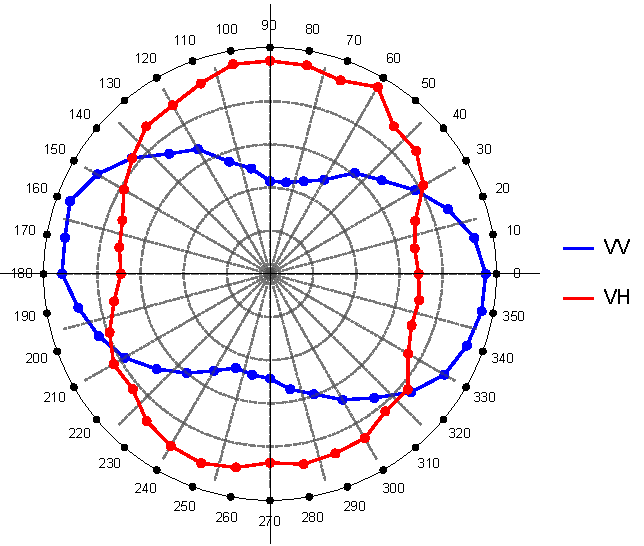
\includegraphics[width=0.75\linewidth]{Wyniki/WidmoPolaryzacyjne/plot390.pdf}
		\caption{Widmo polaryzacyjne dla pika 7 $\rightarrow$ 390$cm^{-1}$ }
	\end{center}
\end{figure}



	\newpage

\section{Opracowanie wyników}

Strukturę $\mathbf{Ga_{2}S_{3}}$ można przedstawić w postaci grup $\mathbf{[GaS_{4}]}$. Siarka jest zlokalizowana na wierzchołkach tetraedru, a gal jest zlokalizowany w środku.

\begin{figure}[H]
	\begin{center}
		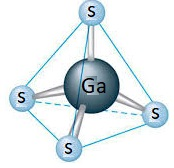
\includegraphics[width=0.3\linewidth]{Opracowanie/tetraedr.jpg}
		\caption{Grupa $\mathbf{Ga_{2}S_{3}}$.}
	\end{center}
\end{figure}

Drania fononów można podzielić na dwie grupy:
\begin{itemize}
	\item Drgania o niskiej energii. Drgania niskoenergetycznych fononów, dla których przesunięcie pików na widmie polaryzacyjnym jest mniejsze od 200 $cm^{-1}$. Do tej grupy należą piki o numerach: 1, 2, 3;
	\item Drgania o wysokiej energii. Drgania wysokoenergetyczne fononów, dla których przesunięcie pików na widmie polaryzacyjnym jest większe od 200 $cm^{-1}$. Do tej grupy należą piki o numerach 4, 5, 6, 7;
\end{itemize}

Częstotliwość drgań można przedstawić za pomocą wzoru:
\begin{equation}
	\omega = \sqrt{\frac{k}{m}}
\end{equation} 

\begin{itemize}
	\item $\omega$ -- częstotliwość drgań;
	\item $k$ -- stałą sprężystości, która zależy od siły oddziaływania między drgającym atomami;
	\item $m$ -- masa atomów.
\end{itemize}

Drgania w ramach jednego tetraedru odpowiada drganiom o wysokiej energii, dla tego że siły wiązania między cząsteczkami w tym samym tetraedrze są duże. Natomiast drgania między cząsteczkami, które się znajdują w różnych tetraedrach są niskoenergetyczne.

Przed rozpoczęciem pomiaru szukaliśmy pod mikroskopem kryształek który przypomina sześciokąt, bo przy pomiarach kryształku w postaci sześciokąta można określić jego osie krystalograficzne.

Chociaż mamy strukturę jednoskośną, przy określonym kierunku kryształ rośnie w postaci sześciokątów. Niżej zostały przedstawione struktury wygenerowane programem VESTA dla struktur $\alpha'$-$Ga_{2}S_{3}$, $\alpha$-$Ga_{2}S_{3}$ i  beta:

\begin{center}
	\begin{figure}[H]
		\begin{minipage}[h]{0.47\linewidth}
			\center{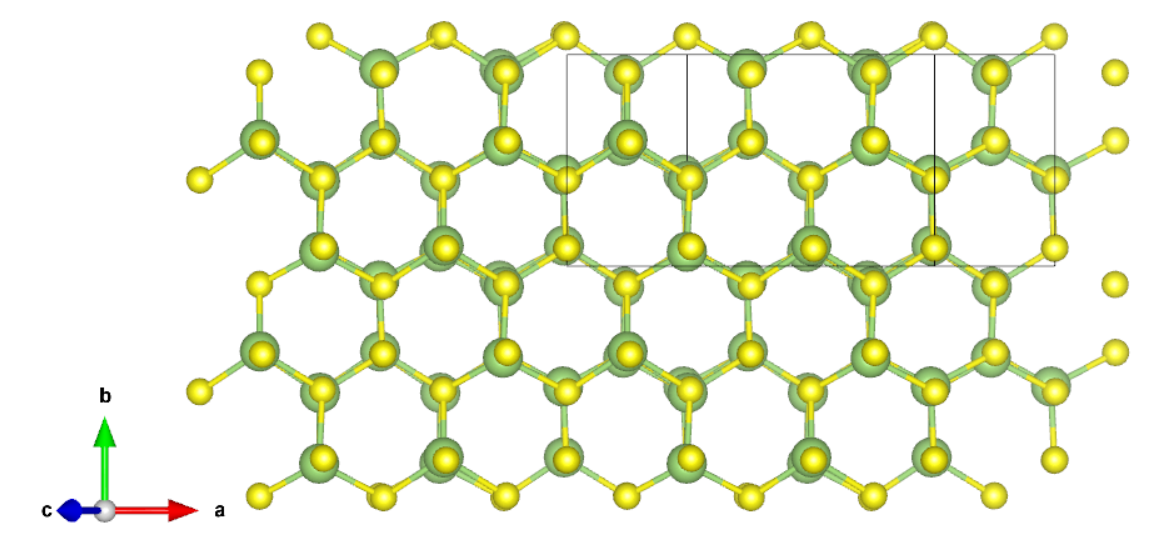
\includegraphics[width=0.8\linewidth]{Opracowanie/alfa_prim_Cc.png}} \\a)
		\end{minipage}
		\hfill
		\begin{minipage}[h]{0.47\linewidth}
			\center{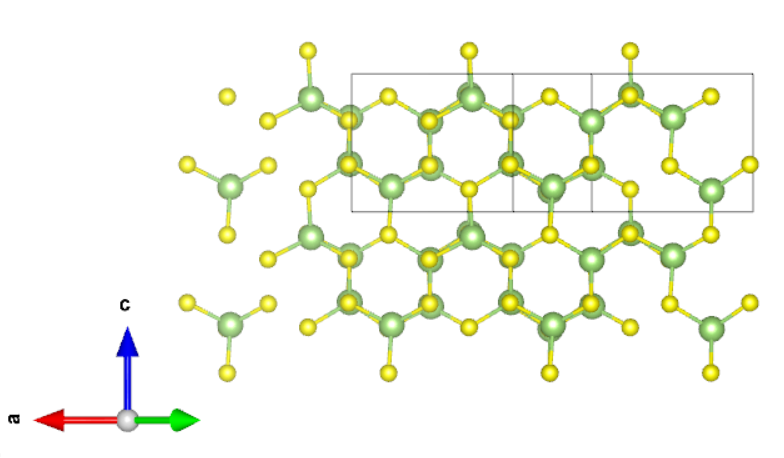
\includegraphics[width=0.8\linewidth]{Opracowanie/alfa_prim_Bb.png}} \\b)
		\end{minipage}
		\caption{a) Struktura krystaliczna $\alpha'$-$\mathbf{Ga_{2}S_{3}}$, grupa przestrzenna Cc. Osie krystalograficzne a i b są prostopadłe i leżą w jednej płaszczyźnie i odpowiadają osiom kartezjańskim x i y. Oś krystalograficzna c jest prostopadła do b i skierowana pod kątem 121$^{\circ}$ do a i skierowana pod kątem 31$^{\circ}$ do osi kartezjańskiej z. b) Struktura krystaliczna $\alpha'$-$\mathbf{Ga_{2}S_{3}}$, grupa przestrzenna Bb. Osie krystalograficzne a i c są prostopadłe i leżą w jednej płaszczyźnie i odpowiadają osiom kartezjańskim x i z. Oś krystalograficzna b jest prostopadła do c i skierowana pod kątem 141$^{\circ}$ do a, i skierowana pod kątem 51$^{\circ}$ do osi kartezjańskiej y. Przygotowano używając oprogramowanie VESTA.[5]}
	\end{figure}
\end{center}

\begin{center}
	\begin{figure}[H]
		\begin{minipage}[h]{0.47\linewidth}
			\center{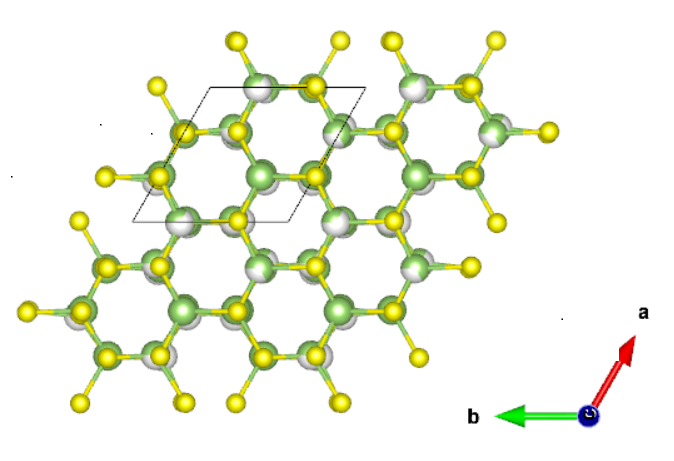
\includegraphics[width=0.8\linewidth]{Opracowanie/alfa.png}} \\a)
		\end{minipage}
		\hfill
		\begin{minipage}[h]{0.47\linewidth}
			\center{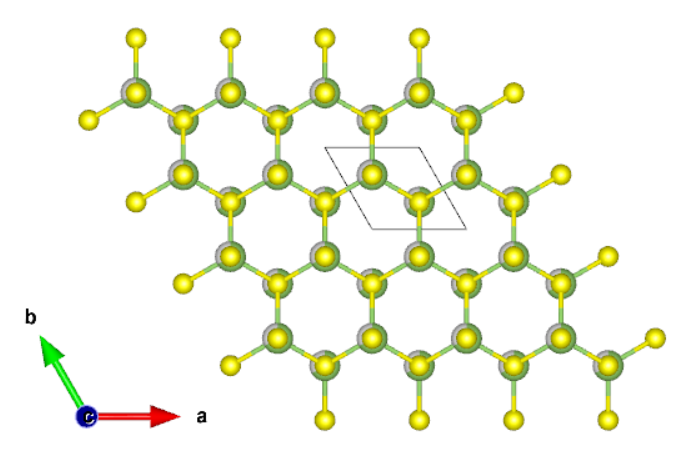
\includegraphics[width=0.8\linewidth]{Opracowanie/beta.png}} \\b)
		\end{minipage}
		\caption{a) Struktura krystaliczna $\alpha$-$\mathbf{Ga_{2}S_{3}}$. Osie krystalograficzne a i b są skierowane pod kątem 120$^{\circ}$ i leżą w jednej płaszczyźnie. Oś krystalograficzna a odpowiada osi kartezjańskiej x, a oś krystalograficzna b jest skierowana pod kątem 30$^{\circ}$ do osi kartezjańskiej y. Oś krystalograficzna c odpowiada osi kartezjańskiej z i jest prostopadła do płaszczyzny w której leżą a i b. b) Struktura krystaliczna $\beta$-$\mathbf{Ga_{2}S_{3}}$. Konfiguracja osi jest taka sama jak w a). Przygotowano używając oprogramowanie VESTA.[5]}
	\end{figure}
\end{center}

Parametrem odpowiedzi modu drgającego na wzbudzenie jest tensor ramanowski, wzór (1). Wektory $e_{i}$ i $e_{s}$ dla naszego układu zależą od jednej z dwóch konfiguracji:
\begin{itemize}
	\item Dla konfiguracji VV wektory mają następującą postać:
	\begin{itemize}
		\item $e_{i} = [\cos \alpha, \sin \alpha, 0]$;
		\item $e_{s} = [\cos \alpha, \sin \alpha, 0]$.
	\end{itemize}
	\item Dla konfiguracji VH wektory mają następującą postać:
	\begin{itemize}
		\item $e_{i} = [\cos \alpha, \sin \alpha, 0]$;
		\item $e_{s} = [-\sin \alpha, \cos \alpha, 0]$.
	\end{itemize}
\end{itemize}

Tensor dla struktury jednoskośnej jest następujący:

\begin{figure}[H]
	\begin{center}
		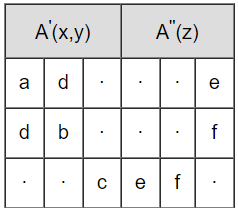
\includegraphics[width=0.3\linewidth]{Opracowanie/Tensor-Cc.png}
		\caption{Tensory ramanowskie dla struktury jednoskośnej.}
	\end{center}
\end{figure}

Dla pików 1, 4, 7 widmo polaryzacyjne dla VH jest przekręcone o kąt 90$^{\circ}$ względem VV. Więc tensor ramanowski dla tych pików przedstawia się jedną macierzą. Ponieważ widmo polaryzacyjne VH nie jest przekręcone o 90$^{\circ}$ dla pozostałych pików, wnioskujemy, że tensor ramanowski dla tych pików jest kombinacją liniową tensorów. 




	\newpage

\section{Podsumowanie}

W ramach tej pracy dokonano przeglądu bogatej literatury dotyczącej materiału $\mathbf{Ga_{2}S_{3}}$, jego własności i zastosowań. Dokonano analizy różnych struktur krystalograficznych $\mathbf{Ga_{2}S_{3}}$, wykorzystując program VESTA i pliki .cif dla danych struktur krystalograficznych $\mathbf{Ga_{2}S_{3}}$.

W cienkiej warstwie $\mathbf{Ga_{2}S_{3}}$ wyhodowanej na $\mathbf{GaP}$ wyselekcjonowano pojedynczy kryształ do badań ramanowskich.
W widmie ramanowskim kryształku siarczku galu wyróżnione zostały 7 pików: 1 $\rightarrow$ 117$cm^{-1}$, 2 $\rightarrow$ 143$cm^{-1}$, 3 $\rightarrow$ 149$cm^{-1}$, 4 $\rightarrow$ 235$cm^{-1}$, 5 $\rightarrow$ 309$cm^{-1}$, 6 $\rightarrow$ 330$cm^{-1}$, 7 $\rightarrow$ 390$cm^{-1}$. Położenia tych pików zgadzało się z danymi literaturowymi. W dalszej części pracy zostały uzyskane i zbadane widma polaryzacyjne dla materiału $\mathbf{Ga_{2}S_{3}}$ dla dwóch różnych konfiguracji: VV i VH. 

W celu określenia zależności natężenia pików ramanowskich od polaryzacji wiązki padającej i rozproszonej wykonano dopasowania do odpowiednich pików przy wykorzystaniu funkcji Voight'a. Zależności polaryzacyjne dla odpowiednich pików zostały przedstawione na wykresach Arrheniusa. Na podstawie przeprowadzonej analizy teoretycznej z wykorzystaniem tensora ramanowskiego wykazano zgodność otrzymanych wyników eksperymentalnych z modelem teoretycznym dla struktury monoclinic $\mathbf{Ga_{2}S_{3}}$.

Zależności polaryzacyjne i dopasowane krzywe zgadzają się z dużą dokładnością. Uzyskane w ramach dopasowania parametry tensora ramanowskiego, odpowiadające modowi A$^{'}$ są następujące:
\begin{itemize}
	\item parametr $a$ przyjmuje wartość 1;
	\item parametr $b$ przyjmuje wartości w granicach 0.67 - 0.80;
	\item parametr $d$ przyjmuje wartości w granicach 0.10 - 0.12.
\end{itemize}

Uzyskane dopasowania pozwalają z dużym prawdopodobieństwem określić, że mamy do czynienia z fazą jednoskośną $\alpha'$-$\mathbf{Ga_{2}S_{3}}$ o grupie przestrzennej Cc.

Wyniki uzyskane w ramach tej pracy były częściowo prezentowane na konferencji EMRS w formie plakatu[37]. Na podstawie bardziej szczegółowych wyników uzyskanych w ramach tej pracy została przygotowana i zgłoszona publikacja w czasopiśmie \textit{Journal: Materials Science in Semiconductor Processing}[1].

%-------------------------

%Na widmie ramanowskim kryształku siarczku galu wyróżnione zostały 7 pików. Dla każdego piku na widmie ramanowskim zostało uzyskane 36 punktów na widmie polaryzacyjnym. Dla pików 1,4,7 została dopasowana pojedyncza funkcja Voigt'a. Dla pików 2 i 3 oraz 5 i 6 została dopasowana podwójna funkcja Voigt'a. W wyniku dopasowania zostały uzyskane parametry tensorów ramanowskich dla poszczególnych pików. 

%<>Dla każdego piku na widmie ramanowskim zostało uzyskane 36 punktów na widmie polaryzacyjnym, obracając co 5 stopni polaryzacją ($"$półfalówką$"$). Dla pików 1,4,7 została dopasowana pojedyncza funkcja Voigt'a. Dla pików 2 i 3 oraz 5 i 6 została dopasowana podwójna funkcja Voigt'a. Uzyskane w wyniku dopasowania pole pod krzywą piku odpowiada natężeniu danego piku ramanowskiego. Na wykresie Arrheniusa naniesione zostały znormalizowane wartości natężeń pików w funkcji konta polaryzacji<>.



	\newpage
 
\addcontentsline{toc}{section}{Bibliografia}
\begin{thebibliography}{}
	\bibitem{litlink1} Cezariusz Jastrzębski, Daniel J. Jastrzebski, Vitali Kozak, Karolina Pietak, Wojciech Gebicki $"$Synthesis and structural characterization of thin $\mathbf{Ga_{2}S_{3}}$ layers on semiconducting $\mathbf{GaP}$ substrate$"$, złożone do Journal: Materials Science in Semiconductor Processing, 2018.
	
	\bibitem{litlink2} $\mathbf{Ga_{2}S_{3}}$ Zeitschrift für Kristallographie - New Crystal Structures, 216, 327-328 (2001)
	
	\bibitem{litlink3} Adrian Kamiński, Instytut Fizyki UAM $"$Spektroskopia Ramana – drgania i widmo rozpraszania$"$
	
	\bibitem{litlink4} Kacper Grodecki1 $"$Spektroskopia ramanowska grafenu$"$
	
	\bibitem{litlink5} Momma K and Izumi F 2011 J. Appl. Crystallogr. 44 1272-1276
	
	\bibitem{litlink6} Ching-Hwa Ho1, Hsin-Hung Chen $"$Optically decomposed near-band-edge structure and excitonic transitions in
	$\mathbf{Ga_{2}S_{3}}$$"$ Sci. Rep. 4, 6143; DOI:10.1038/srep06143
	(2014).
	
	\bibitem{litlink7} H. F. Liu, K. K. Ansah Antwi, N. L. Yakovlev, H. R. Tan, L. T. Ong, S. J. Chua, D. Z. Chi $"$Synthesis and Phase Evolutions in Layered Structure of $\mathbf{Ga_{2}S_{3}}$ Semiconductor Thin Films on Epiready $\mathbf{GaAs}$ (111) Substrates$"$ ACS Appl. Mater. Interfaces 2014, 6, 3501-3507
	
	\bibitem{litlink8} Chang-Sun Yoon, F. D. Medina, L. Martinez, Tae-Young Park, Moon-Seog Jin, and Wha-Tek Kim $"$Blue photoluminescence of $\mathbf{\alpha-Ga_{2}S_{3}}$ and $\mathbf{\alpha-Ga_{2}S_{3}}:Fe^{2+} $sinle crystals$"$ Appl. Phys. Lett. 83, 1947 (2003)
	
	\bibitem{litlink9} I. Gulera,, M. Isik b, L. Gasanovac, A. Mahammadovc, N. Gasanly $"$Thermoluminescence in gallium sesquisulfide single crystals:
	usual and unusual heating rate dependencies$"$ Optik 165 (2018) 132–136
	
	\bibitem{litlink10} K.A. Kokh, Z.M. Huang, J.G. Huang, Y.Q. Gao, B. Uralbekov, J. Panomarev, I.N. Lapin, V.A. Svetlichnyi, G.V. Lanskii, Yu. M. Andreev $"$Study of $\mathbf{Ga_{2}S_{3}}$ crystals grown from melt and $\mathbf{PbCl_{2}}$ flux$"$ Materials Research Bulletin 84 (2016) 462–467
	
	\bibitem{litlink11} Tansir Ahamad and Saad M Alshehri $"$Green Synthesis and Characterization of Gallium(III) Sulphide $\mathbf{Ga_{2}S_{3}}$
	Nanoparicles at Room Temperature$"$ Nano Hybrids Vol. 6 (2014) 37-46
	
	\bibitem{litlink12} I. Carman, D. Rusu, E.R. Ardeleanu, I.Evtodiev $"$THE Detectors of UV and X radiation based on $\mathbf{Ga_{2}S_{3}}$ and $\mathbf{GaSe}$ semiconductors intercalated with $\mathbf{Cd}$$"$ Vol. 7, No. 1, January - March 2015, p. 27 - 32
	
	\bibitem{litlink13} H. F. Li K. K. Ansah Antw C. S. Chu J. Huang S. J. Chu and D. Z. Chia $"$Epitaxial Synthesis, Band Offset, and Photoelectrochemical
	Properties of Cubic $\mathbf{Ga_{2}S_{3}}$ Thin Films on $\mathbf{GaAs}$ (111) Substrates$"$ ECS Solid State Letters, 3 (11) P131-P135 (2014)
	 
	\bibitem{litlink14} Katerina M Othonos, Matthew Zervos, Constantinos Christofides and Andreas Othonos $"$Ultrafast Spectroscopy and Red Emission
	from $\beta-\mathbf{Ga_{2}O_{3}}/ \beta-\mathbf{Ga_{2}S_{3}}$ Nanowires$"$ Othonos et al. Nanoscale Research Letters (2015) 10:304
	
	\bibitem{litlink15} Ching-Hwa Ho, Min-Han Lin, Yi-Ping Wang, Ying-Sheng Huang $"$Synthesis of $\mathbf{In_{2}S_{3}}$ and $\mathbf{Ga_{2}S_{3}}$ crystals for oxygen sensing and UV photodetection$"$ Sensors and Actuators A 245 (2016) 119–126
	
	\bibitem{litlink16} S. R. Alharbi, A. F. Qasrawi $"$Dielectric Dispersion in $\mathbf{Ga_{2}S_{3}}$ Thin Films$"$ Plasmonics (2017) 12:1045–1049
	
	\bibitem{litlink17} A. N. Georgobiani, B. G. Tagiev, O. B. Tagiev, Kh. B. Ganbarova, and U. F. Kasumov $"$Photoluminescence and Raman Spectra of $\mathbf{(Ga_{2}S_{3})_{0.95}(Sm_{2}O_{3})_{0.05}} Crystals$$"$ Neorganicheskie Materialy, 2010, Vol. 46, No. 10, pp. 1172–1174.
	
	\bibitem{litlink18} I. Pethes, V. Nazabal, R. Chahal, B. Bureau, I, Kaban, S. Belin, P. Jówari $"$Local motifs in $\mathbf{GeS_{2}-Ga_{2}S_{3}}$ glasses$"$
	
	\bibitem{litlink19} S. Caramazza A. Collina, E. Stellino, P. Dore, and P. Postorino $"$Polarization analysis of first- and second-order Raman scattering from $\mathbf{MoTe_{2}}$ single crystal.$"$
	
	\bibitem{litlink20} Guihua Shang, Mark J. Hampden-Smith and Eileen N. Duesler $"$Synthesis and characterization of gallium thiocarboxylates as novel single-source precursors to gallium sulfide thin films by aerosol-assisted CVD$"$ Chem. Commun., 1996
	
	\bibitem{litlink21} Mike R. Lazel, Paul O’Brien, David J. Otway, and Jin-Ho Park $"$Deposition of Thin Films of Gallium Sulfide from a Novel Single-Source
	Precursor, $\mathbf{Ga(S_{2}CNMeHex)_{3}}$, by Low-Pressure Metal-Organic Chemical Vapor Deposition$"$ Chem. Mater. 1999, 11, 3430-3432
	
	\bibitem{litlink22} V.P. Mushjnskii, L.I. Palaki, and V.V. Chebotaru $"$Optical Absorption $\alpha-Ga_{2}S_{3}$ Single Crystals$"$ phys. stat. sol. (b) 83, K149 (1977)
	
	\bibitem{litlink23} A. Tomas, M. Guymon, M.P. Pardo, M. Guittard, and J. Flahau $"$X-Ray Diffraction and Electron Microscopy Studies of $\alpha-$ and $\beta$-$\mathbf{Ga_{2}S_{3}}$$"$ phys. stat. sol. (a) 107, 775 (1988)
	
	\bibitem{litlink24} Huseyin Ertap, Tarik Baydar, Mustafa Yuksek, Mevlut Karabulut $"$Structural and optical properties of gallium sulfide thin film$"$ Turk J Phys (2016) 40: 297-303
	
	\bibitem{litlink25} Zhiming Huang, J.-G. Huang, K.A. Kokh,c, V.A. Svetlichnyi, A.V. Shabalina, Yu.M. Andreev, and G.V. Lanskii. $"$$\mathbf{Ga_{2}S_{3}}$ - optical properties and perspectives for THz applications$"$
	 
	\bibitem{litlink26} Racoveţ O., Evtodiev I., Caraman Iu., Rotaru I, Lazăr G.
	$"$Optical Properties of Compounds with submicron points otained
	through $\mathbf{Ga_{2}S_{3}}$ intercalation with $\mathbf{Cd}$$"$  Procese, modele, experimente, nr. 2, 2012
	
	\bibitem{litlink27} Andrew R. Barron $"$Chalcogenides of Aluminum,
	Gallium, and Indium$"$ OpenStax-CNX module: m33044
	
	\bibitem{lilink28} J. Thorstensen, K. H. Haugholt, A. Ferber, K. A. H. Bakke, J. Tschudi $"$Low-cost resonant cavity Raman gas probe for multi-gas
	detection$"$ J. Europ. Opt. Soc. Rap. Public. 9, 14054 (2014)
	
	\bibitem{litlink29} C.Y. Jones J.C. Bryan, K. Kirschbaum and J. G. Edwards $"$Refinement of the crystal structure of digallium trisulfide, $\mathbf{Ga_{2}S_{3}}$$"$ Z. Kristallogr. NCS 216 (2001) 327-328
	
	\bibitem{litlink30} Christian Kranert, Chris Sturm, Rüdiger Schmidt-Grund and Marius Grundmann $"$Raman tensor elements of $\beta$-$\mathbf{Ga_{2}O_{3}}$$"$ Scientific Reports | 6:35964 | DOI: 10.1038/srep35964
	 
	\bibitem{litlink31} Tao Haizheng, Zhao Xiujian, Jing Chengbin, Yang Hui, Mao Shun $"$Raman scattering studies of the $\mathbf{GeS_{2}-Ga_{2}S_{3}-CsCl}$$"$ Solid State Communications 133 (2005) 327-332.
	
	\bibitem{litlink32} R. Rao, H. Chandrasekaran, S. Gubbala, M.K. Sunkara,
	C. Daraio, S. Jin, and A.M. Rao $"$Synthesis of Low-Melting Metal Oxide and
	Sulfide Nanowires and Nanobelts.$"$ Journal of ELECTRONIC MATERIALS, Vol. 35, No. 5, 2006
	
	\bibitem{litlink33} E.M. Marmolejo, E. Granado, O.L. Alves, C.L. Cesar, L.C. Barbosa $"$Spectroscopy and thermal properties of $\mathbf{Ga_{2}S_{3}}$ based glasses$"$ Journal of Non-Crystalline Solids 247 (1999) 189-195
	
	\bibitem{litlink34} Katerina M Othonos, Matthew Zervos, Constantinos Christofides and Andreas Othonos $"$Ultrafast Spectroscopy and Red Emission
	from $\beta-\mathbf{Ga_{2}O_{3}}/\beta-\mathbf{Ga_{2}S_{3}}$ Nanowires$"$ Othonos et al. Nanoscale Research Letters (2015) 10:304
	
	\bibitem{litlink35} Eman O. Nazzal, A. F. Qasrawi, S. R. Alharbi $"$Engineering the Optical and Dielectric Properties
	of the $\mathbf{Ga_{2}S_{3}/In/Ga_{2}S_{3}}$ Nanosandwiches via Indium Layer
	Thickness$"$
	
	\bibitem{litlink36} Jastrzębski Daniel, Praca inżynierska, Wydział Chemii Politechniki Warszawskiej, promotor prof. dr hab. inż. Sławomir Podsiadło
	
	\bibitem{litlink37} Daniel J. Jastrzebski, Karolina Pietak, Cezariusz Jastrzebski, Slawomir Podsiadlo, Syntesis of thin Ga2S3 layers on semiconducting substrates, EMRS, Fall Meeting 2018, Poster, Book of abstracts, \textbf{R.P2.13}
	
\end{thebibliography}















\end{document}
